%&preamble
%Einbinden des vorkompilierten Preambles, bei Änderungen Ausführen von /preamble.bat 
%\PassOptionsToPackage{svgnames}{xcolor} %farbige blöcke
\documentclass[
%DIV = calc, %automatische Berechnung vonsseitenrändern
10pt,
a4paper,
oneside,
bibliography=totoc,         %vorher bibtotoc
listof=totoc,               %vorher liststotoc
headsepline, 
headings=small,             %vorher smallheadings
openright, 
fleqn,
appendixprefix,
draft,
BCOR=5mm,                   %vorher BCOR5mm
]
{scrbook}

%%Pfadprüfung%%
\IfFileExists{../../_preamble/check_file.tex}% Prüfung aus welcher Datei der Aufruf stattfindet
{%
\providecommand{\myPath}{../../}% file exists=true: befinde mich im Unterverzeichnis
}%
{%
\providecommand{\myPath}{}% file exists=false: befinde mich im RootVerzeichnis
}%
%%Pfadprüfung%%

%%Einbinden globaler Pakete und Paketeinstellungen%%
%//Allgemeine Pakete\\%
\usepackage[utf8]{inputenc}				% OK, Korrektes Encoding in Latex-Schrift, 							check: 25.08.18
\usepackage[ngerman]{babel}				% OK, Korrekte Schreibweise und Treenungsregelung					check: 25.08.18
\usepackage[T1]{fontenc}				% OK, Korrektes Font-Encoding			 							check: 25.08.18
\usepackage{amsmath} 					% OK, Mathematische Symbole und Schriften, 							check: 25.08.18
\usepackage{amsfonts} 					% OK, Mathematische Symbole und Schriften, 							check: 25.08.18
\usepackage{amssymb} 					% OK, Mathematische Symbole und Schriften, 							check: 25.08.18
\usepackage{amsthm} 					% OK, Typesetting Theoreme, 										check: 25.08.18
\usepackage{exscale}  					% OK, Skalierung von mathematischen Symbolen, 						check: 25.08.18
\usepackage{amstext} 					% OK, Text in mathematischer Umgebung, 								check: 25.08.18 [enthalten in amsmath]
\usepackage{verbatim} 					% OK, Funktion zum Schreiben von unformatiertem Text, 				check: 25.08.18
\usepackage{float} 						% OK, Ermöglicht das Erstellen von eigenen Float Umgebungen, 		check: 25.08.18
%\usepackage{makeidx}					% OK, Erstellen von Indizes zur Anlegung eines Glossars, 			check: 25.08.18
\usepackage{standalone} 				% OK, Kompilierung als eigenes Dok und Einbindung über Main,		check: 25.08.18
%\usepackage{import} 					% OK, Übernahme von relativen Verweisen in \inputs,					check: 25.08.18


%//Syntaktische Formatierung\\%
\usepackage{scrlayer-scrpage}			% OK, Definition und Manipulation von Kopf-, Fußzeile,				check: 25.08.18
\usepackage[onehalfspacing]{setspace}	% OK, Einstellen Zeilenabstand (onehalfspacing, doublespacing)		check: 25.08.18
\usepackage[							% OK, Definition des Seitenlayouts,									check: 25.08.18
includeheadfoot,						%
left=3cm,right=2cm,top=2cm,bottom=2cm,	%
showframe								%
]{geometry}								%
\usepackage[section]{placeins} 			% OK, Verhindert das Wandern von floats in eine andere section, 	check: 25.08.18
\usepackage{microtype} 					% OK, Abstand zwischen Zeichen anpassen zur Darstellung,			check: 25.08.18
\usepackage{lmodern}					% OK, Latin Modern font,											check: 25.08.18


%//Bilder und Tabellen\\%
\usepackage{xcolor} 					% OK, Definieren und Nutzen von versch. Farben						check: 25.08.18
\usepackage{graphicx}					% OK, Bereitstellen von \includegraphics							check: 25.08.18
\usepackage{array} 						% OK, Erstellen eigener Columntypen in Tabellenumgebungen			check: 25.08.18
\usepackage{rotating} 					% OK, Rotieren von floats in boxen (Tabellen, Bilder)				check: 25.08.18
\usepackage{adjustbox}					% OK, Ähnlich wie resizebox für normale Textumgebung,				check: 25.08.18
\usepackage{booktabs}					% OK, Schönere Tabellen ohne vertikale Linien \toprule etc.			check: 25.08.18
\usepackage{tabularx}					% OK, Weiterer Spaltentyp passt Tabellenbreite  automatisch an		check: 25.08.18
\usepackage{multirow}					% OK, Zellenspannung über mehrere Zeilen							check: 25.08.18
%\usepackage{makecell}					% OK, Tabellenlayout (Tabaellenheader) ähnlich \multirow			check: 25.08.18
\usepackage{tablefootnote}				% OK, Fußnoten in Tabellen (\footnote funktioniert nicht)			check: 25.08.18
\usepackage{subcaption} 				% OK, Darstellung von Tabellenumgebungen aus mehreren (auch Figure)	check: 25.08.18


%//Diverses\\%
\usepackage{paralist} 					% OK, Aufzählung wie \itemize \compactenum (nochmal anschauen)		check: 25.08.18
\usepackage[withpage]{acronym}			% OK, Genutze Abkürzungen werden das erste mal ausgeschrieben		check: 25.08.18
\usepackage{fancybox}					% OK, Verschiedene Varianten von \fbox zur Umrahmung von Text		check: 25.08.18
\usepackage[most]{tcolorbox}			% OK, Colorierte und umrahmte Textboxen wie \fbox für Theoreme		check: 25.08.18
\usepackage{layouts}					% OK, Darstellen von Dokumenteninformationen,						check: 25.08.18
%\usepackage[textsize=tiny]{todonotes}	% OK, Markierung und Erstellung von todo-Anmerkungen				check: 25.08.18
%\usepackage[timer]{regstats}			% Keine Funktion?, Erhebung von Statistiken (Kompiluierungszeit)	check: 25.08.18
%\usepackage[l2tabu, orthodox]{nag}		% Keine Funktion?, Prüfung nach veralteten Paketen					check: 25.08.18


%//Theoreme\\%
%\usepackage{ntheorem} 					% OK, Darstellung von Theoremen										check: 25.08.18
%\usepackage{thm­tools} 				% OK, Darstellung von Theoremen <-									check: 25.08.18
\newtcbtheorem[number within=section, list inside=def]{mydef}{Definition}%
{enhanced, colback=white,colframe=\fillTwo,fonttitle=\bfseries, description delimiters={\flqq}{\frqq}, description font=\mdseries\ttfamily, boxrule=0.4pt,toprule=3pt, boxsep=3pt,arc=0mm, list text={test}, drop shadow}{def}


%//Zitate und Links\\%
\usepackage{csquotes}					% OK, Korrekte Darstellung von "" je nach Land						check: 25.08.18
\usepackage[]{hyperref}					% OK, Cross-Referencing und hypermarks im Dokument					check: 25.08.18
\hypersetup{
bookmarksopen=true,
pdfpagelabels=true,
plainpages=false,
colorlinks=true,
citecolor=blue,
linkcolor=blue,
urlcolor=blue}

%//BibLatex\\%
\usepackage[backend=biber,				% OK, Neue Version von BibTex zur Darstellung Literaturverzeichnis	check: 25.08.18 
style=authoryear, %% Zitierstil
natbib=true, %% Bereitstellen von natbib-kompatiblen Zitierkommandos
hyperref=true, %% hyperref-Paket verwenden, um Links zu erstellen
maxcitenames=1,
uniquelist=false,
bibstyle=numeric,
url=false,
doi=false
]{biblatex}
%\addbibresource{bibfile.bib} 			% Einbinden der bib-Datei
%\DefineBibliographyStrings{ngerman}{andothers={et al.}} % et al. statt u.a.
%\renewcommand*{\nameyeardelim}{\addcomma\space} % Macht im Zitat ein Komma vor das Jahr
%%Font etc.%%
\usepackage{lmodern}					% OK, Latin Modern font,											check: 25.08.18
\usepackage{xcolor} 					% OK, Definieren und Nutzen von versch. Farben						check: 25.08.18
\usepackage{graphicx}					% OK, Bereitstellen von \includegraphics							check: 25.08.18

%%Forest%%
\usepackage{forest}						% OK, Baumdarstellung aus dem linguistischen Bereich				check: 25.08.18
\useforestlibrary{edges}

%%Venndiagramm%%
\usepackage{venndiagram}				% OK, Definieren und Darstellen von Venndiagrammen					check: 25.08.18

%%Tabellen%%
\usepackage{booktabs}					% OK, Schönere Tabellen ohne vertikale Linien \toprule etc.			check: 25.08.18
\usepackage{tabularx}					% OK, Weiterer Spaltentyp passt Tabellenbreite  automatisch an		check: 25.08.18
\usepackage{multirow}					% OK, Zellenspannung über mehrere Zeilen							check: 25.08.18
%\usepackage{makecell}					% OK, Tabellenlayout (Tabaellenheader) ähnlich \multirow			check: 25.08.18
\usepackage{tablefootnote}				% OK, Fußnoten in Tabellen (\footnote funktioniert nicht)			check: 25.08.18
\usepackage{array} 						% OK, Erstellen eigener Columntypen in Tabellenumgebungen			check: 25.08.18

%%Grafiken und Plots%%
\usepackage{tikz} 						% OK, Natives zeichnen in Latex ,									check: 25.08.18
\usepackage{tikz-cd} 					% OK, Erstellen von kommutativen Diagrammen in Tikz,				check: 25.08.18
\usepackage{pgfplots}					% OK, Plotten von Daten,											check: 25.08.18
\pgfplotsset{compat=newest}				% OK, Einstellen der Kompatibilitätsversion,						check: 25.08.18
\usepackage{pgfplotstable}				% OK, Plotten und schreiben von Daten in Tabellen,					check: 25.08.18
\usepackage{pgfcalendar} 				% OK, Umrechnen von Datumskoordinaten,								check: 25.08.18
\usepgfplotslibrary{dateplot}			% OK, Plotten von Datumskoordinaten,								check: 25.08.18
\usepgfplotslibrary{units}				% OK, Darstellen von Einheiten als Achsenlabel,						check: 25.08.18
%//Tikzbibliotheken\\%
\usetikzlibrary{						% Bibliotheken zur direkten Einbindung in TIKZEdt
arrows, 
fit,
shapes.geometric, 
matrix,
calc,
decorations.markings,
decorations.pathreplacing,
decorations.pathmorphing,
backgrounds,
shadings, 
shadows,
positioning,
mindmap,
trees,
datavisualization
}
%%Einbinden globaler Pakete und Paketeinstellungen%%

\endofdump %% <-- Precompile bis hierhin 

%%Einbinden globaler Stile uns Einstellungen%%
%%define tikz-stlyes here, colours etc.
\tikzset{
block_phantom/.style={block_normal, draw=red, fill=none},
block_phantom/.style={block_normal, draw=blue, fill=none}
}
%\tikzstyle{block_phantom}=[block_normal, draw=red, fill=none]
\pgfplotsset{
  global_appearance/.style={
  grid_appearance,
  scale only axis,
  width= .75\textwidth,
  %width=12.5cm, % 13,5
  height=.4\textwidth
  }
}

\pgfplotsset{
  grid_appearance/.style={
   grid,
   grid style = {loosely dotted , thin},
  }
}

\pgfplotsset{
 %every axis plot/.append style={no markers},
  every pin/.append style={font=\footnotesize },
  every mark/.append style={scale=3},
  legend style=
  {
  font=\tiny, 
  %draw=none, 
  cells={align=left}, 
  at={(0.5,1.00)},
  anchor=north,
 % legend pos= north west
  },
  legend columns = 2,
  label style={font=\scriptsize},
  tick label style={font=\tiny},
}

\pgfplotsset{
  tuftle_like_axes/.style={
  thin,  %vorher semithick
  tick style={major tick length=4pt,thin,black}, %vorher semithick
  separate axis lines,
  axis x line*=bottom,
  axis x line shift=10pt,
  xlabel shift=5pt,
  axis y line*=left,
  axis y line shift=10pt,
  tick align = outside,
  ylabel shift=2pt,
  enlarge y limits=false,
  enlarge x limits=false,
  }
}

%%Tufte-Design%%
% \makeatletter
% \pgfplotsset{
  % tufte axes/.style =
    % {
      % after end axis/.code =
        % {
          % \draw ({rel axis cs:0,0} -| {axis cs:\pgfplots@data@xmin,0}) -- ({rel axis cs:0,0}  -| {axis cs:\pgfplots@data@xmax,0});
          % \draw ({rel axis cs:0,0} |- {axis cs:0,\pgfplots@data@ymin}) -- ({rel axis cs:0,0}  |-{axis cs:0,\pgfplots@data@ymax});
        % },
      % axis line style = {draw = none},
      % tick align      = outside,
      % tick pos        = left
    % }
% }
% \makeatother
%//Commands\\%
\newcommand{\fillOne}{green!35!black}						% Farbenneudefinition	
\newcommand{\fillTwo}{black!70}								% Farbenneudefinition	
\newcommand{\fillThree}{blue!30!}							% Farbenneudefinition	
\newcommand{\fillFour}{black!10!blue}						% Farbenneudefinition	

\newlength{\freewidth}										% Zur Berechnung noch freien Platzes bei prozentualer Angabe der Spaltenbreite in Tabellen

%//Settings\\%
\setcounter{secnumdepth}{3}									% Sektionstiefe definieren zur Darstellung im Inhaltsverzeichnis		
\setcounter{tocdepth}{4}									% Tiefe definieren zur Darstellung im Inhaltsverzeichnis

\renewcommand{\topfraction}{0.85} 							% Anteil einer Seite, die von Floats belegt sein darf (default 0.7)
\renewcommand{\textfraction}{0.1} 							% Anteil einer Seite, die mindestens Text sein muss (default 0.2)
\renewcommand{\floatpagefraction}{0.75} 					% Anteil einer Seite, die ein Float einnehmen darf, ohne auf die nächste Seite gesetzt zu werden (default 0.5)	

\newtheorem{theorem}{Satz}									% Theorem Satz
\newtheorem{definition}{Definition}							% Theorem Definition <-
\newtheorem{lemma}{Lemma}									% Theorem Lemma

\newcolumntype{L}[1]{>{\raggedright\arraybackslash}p{#1}} 	% Linksbündig mit Breitenangabe
\newcolumntype{C}[1]{>{\centering\arraybackslash}p{#1}} 	% Zentriert mit Breitenangabe
\newcolumntype{R}[1]{>{\raggedleft\arraybackslash}p{#1}} 	% Rechtsbündig mit Breitenangabe
%\newcolumntype{C}[1]{>{\centering\arraybackslash}m{#1}} 	% Vertikale zentrierung

\captionsetup[figure]{										% Captionsetup für Figure-Umgebung
%skip=5cm,
position=below,
justification=centering,
font=small
}
\captionsetup[table]{										% Captionsetup für Tabellen-Umgebung
%skip=5cm,
position=below,
justification=centering,
font=small}
\setlength\abovecaptionskip{10pt}
\setlength\belowcaptionskip{10pt}





%%Einbinden globaler Stile und Einstellungen%%


\begin{document}

%% Ausgabe Dokumenteneigenschaften
%% display some document properties

\edef\defaultfont{\fontname\font}  % Speichert die Default Font inkl. Schriftgrad
\edef\defaultsize{\csname f@size\endcsname}  % Speichert die Default Font inkl. Schriftgrad
\newcommand{\currentfont}{\fontname\font}
\newcommand{\currentsize}{\csname f@size\endcsname}

\begin{table}[]
\footnotesize
\centering
\setlength{\freewidth}{\dimexpr\textwidth-6\tabcolsep}
\begin{tabular}{L{.8\freewidth}L{.1\freewidth}L{.10\freewidth}}   % 100% without resizbox
\toprule
Feature & Value \\
\midrule
PaperWidth in [cm]& \printinunitsof{cm}\prntlen{\paperwidth}\\
PaperHeight in [cm]& \printinunitsof{cm}\prntlen{\paperheight}\\
TextWidth in [cm] &  \printinunitsof{cm}\prntlen{\textwidth}  \\
TextHeight in [cm] & \printinunitsof{cm}\prntlen{\textheight}\\
\midrule
MarginParSep in [cm] & \printinunitsof{cm}\prntlen{\marginparsep}\\
MarginParWidth in [cm] & \printinunitsof{cm}\prntlen{\marginparwidth}\\
FootSkip in [cm]& \printinunitsof{cm}\prntlen{\footskip}\\
\midrule
Default Font &  \defaultfont \\
Default Size   & \defaultsize \\
Current Font &  \currentfont \\
Current Size &  \currentsize \\
\midrule
Colour1 & \fillOne & \begin{tikzpicture} \draw[fill=\fillOne, draw=none] (0,0) rectangle (1,.2); \end{tikzpicture}\\
Colour2 & \fillTwo & \begin{tikzpicture} \draw[fill=\fillTwo, draw=none] (0,0) rectangle (1,.2); \end{tikzpicture}\\
Colour3 & \fillThree & \begin{tikzpicture} \draw[fill=\fillThree, draw=none] (0,0) rectangle (1,.2); \end{tikzpicture}\\
Colour4 & \fillFour & \begin{tikzpicture} \draw[fill=\fillFour, draw=none] (0,0) rectangle (1,.2); \end{tikzpicture}\\
\bottomrule 
\end{tabular}
\end{table}

%% Ausgabe Dokumenteneigenschaften

\begin{onehalfspace} %Start 1,5-facher Zeilenabstand
\pagestyle{empty}
\pagenumbering{alph}
%//Metadaten\\%
\newcommand{\logo}{
	
\includegraphics[width=0.6\textwidth]{_img/_pdf/Logo_Uni_Paderborn}\\
}
\newcommand{\fachbereich}{
	\begin{tabular}{c}
	Fachgebiet Wirtschaftsinformatik   \\
	Information Management \& E-Finance  \\
	Prof. Dr. Dennis Kundisch    \\
	Universität Paderborn   \\
	\end{tabular}
}
\newcommand{\titel}{
	Experimente in der Wirtschaftsinformatik zu Kreativität: Ein
	Systematischer Literaturüberblick und Implikationen für
	Geschäftsmodell-\\modellierungstools
}
\newcommand{\vorgelegtvon}{
	vorgelegt im Rahmen der Abschlussprüfung\\
	für den Bachelor-Studiengang\\
	der Wirtschaftsinformatik
}
\newcommand{\autorpruefer}{
	\begin{tabular}{ll}
      Autor: & xxx xxx \\
      Matr.-Nr.: & xxxxxx\\
      Adresse: & xxxxxx xxxxxx xxx\\
      & 33098 Paderborn\\
      E-Mail: & xxxxxx@mail.upb.de\\
      &\\
      &\\
      Erstprüfer: & Prof. Dr. Dennis Kundisch \\
      Zweitprüfer: & Prof. Dr. Leena Suhl \\
      Betreuer: & Daniel Szopinski \\
	\end{tabular}
}
\newcommand{\datum}{
	Paderborn, den \today
}

\begin{titlepage}
\singlespacing
\centering

\logo
\vspace{1cm}

\fachbereich \par
\vspace{2cm}

{\scshape\huge Bachelorarbeit \par}
\vspace{1.5cm}

{\LARGE\bfseries \titel \par}
\vspace{2cm}

\vorgelegtvon \par
\vspace{2cm}

{\autorpruefer \par}
\vfill

\datum
\end{titlepage}
 \cleardoublepage
\noindent
Hiermit erkläre ich an Eides Statt, dass ich die vorliegende Arbeit selbständig und ohne unerlaubte fremde Hilfe angefertigt, andere als die angegebenen Quellen und Hilfsmittel nicht benutzt und die den benutzten Quellen und Hilfsmitteln wörtlich oder inhaltlich entnommenen Stellen als solche kenntlich gemacht habe.\\
\\
\\
Paderborn, \today
\begin{flushright}
------------------------------------------\\
(Vorname Name)
\end{flushright}
 \cleardoublepage
\section*{Abstract - deutsch}
Der Forschungsberich der Wirtschatfsinformatik wird im wesentlichen von Artefakten geprägt. Im Zyklus der Artefaktentwicklung stellt deren Evaluierung ein fest definierter Schritt dar. Experimente bilden auf dieser Grundlage ine geeignete Möglichkeit zur Durchführung dieser Evlauierung.  Zeitgleich fordert die betriebswirtschaftliche Komponente der Wirtschaftsinformatik im Bereich der Geschäftsmodellentwicklung neue Erkentnisse, indem die Wichtigkeit der Entwicklungs- und Implementierungsunterstützzung neuer Geschäftsmodelle  vorangetrieben werden sollen. Dazu eignen sich die im Rahmend er Gestaltungsorientieren WI entwickelten Artefakte als Unterstützung in diesem kreativen Schaffensprozess.  Diese Arbeit nimmt sich das Ziel der Literaturüberischt, wie sich solche Artefakte im Gebiet der Kreativitätsforschung im Rahmen des Evaluierungsprozesses durch Experimente überprüft werden. Dazu wurden 850 Paper analysiret, deren Zahl sich nach Auswertung auf 50 reduzierte. Anahnd dieser Arbeiten wird eine vergleichende Strukturanalyse vorgenommen die es ermöglicht einen Überblick über das experimetnelöle Vorgehensweisen in diesem Bereich zu erlangen. Die Ergebnisse zeigen, dass ein großteil der Experimenten RQ1 ….. Basierend auf den gesammelten Informationen der Durchführung wurde untersucht, ob sich aus den Methodenwissen aus Experiment und Kreativitätsforschung bbereits Implikationen für die Entwicklung von GMMT ableiten lassen. RQ2…..  \\\\
Stichworte: experiment, kreativität, literatur review, creativity support system, geschäftsmodellmodellierungstool

\section*{Abstract - englisch}
Eine Zusammenfassung der Arbeit in englischer Sprache.
\\\\
Keywords: experiment, creativity, design science research, literature review, creativity support system, businessmodelmodellingtool 
\\\\\\



 \cleardoublepage
\clearpage
\thispagestyle{empty}
\null\vfill
\begin{center}
{\scshape\huge Vorwort \par}
\end{center}
\vspace{.5cm}
\addcontentsline{toc}{chapter}{Vorwort}
Die vorliegende Arbeit soll einen Beitrag zum Projektbereich Softwarebasierte Geschäftsmodellmodellierungstools: Theorie und empirische Beweise der Universität Paderborn leisten. Da innerhalb des Projektes die evidente Experimentelle Forschung ein Hauptaugen,ekr ist, wird in dieser Arbeit ein Überblick geschaffen, indem Wissen aus der experimentellen Forschung sowohl im Bereich der Kreativität als auch der Wortschaftsinformatik untersucht und sysnthetisiert wird.

\vfill
\clearpage
 \cleardoublepage
\pagestyle{scrheadings}
\frontmatter
\tableofcontents \cleardoublepage
%\addcontentsline{toc}{chapter}{\listfigurename}
 \listoffigures \cleardoublepage
%\listofalgorithms \cleardoublepage
\listoftables \cleardoublepage
%\tcblistof[\chapter]{def}{Definitionsverzeichnis}\cleardoublepage
%\listoftodos \cleardoublepage
\addchap{Abkürzungsverzeichnis}
%\phantomsection \addcontentsline{toc}{chapter}{Abkürzungsverzeichnis}
%\renewcommand\refname{Abkürzungsverzeichnis} \chapter*{Abkürzungsverzeichnis}
\begin{acronym}[Bashgfgfdgfdgfd]
 \acro{KDE}{K Desktop Environment}
 \acro{SQL}{Structured Query Language}
 \acro{Bash}{Bourne-again shell}
 \acro{JDK}{Java Development Kit}
 \acro{VM}{Virtuelle Maschine}
 \acro{I2C}{Inter-Integrated Circuit}
\end{acronym}
 \cleardoublepage

%//Ausprobieren\\%
%\newfloat{ergebnisse}{thb}{loh}[chapter] % Liste der detaillierten Ergebnisse
%\floatname{ergebnisse}{Ergebnisse}
%\listof{ergebnisse}{Liste der detaillierten Ergebnisse}
%\cleardoublepage
%//Ausprobieren\\%


\mainmatter % der eigentliche Text folgt hier
\chapter{Einleitung}
\begin{singlespace}
\renewcommand*{\dictumwidth}{0.4\textwidth} 
\dictum[Richard Phillips Feynman \footnotemark]{It doesn't matter how beautiful your theory is, it doesn't matter how smart you are. If it doesn't agree with experiment, it's wrong.}
\footnotetext{1964, Transkipt der Messenger Lectures an der Cornell Universität: The Character of Physical Law}\bigskip 
\end{singlespace}

\section{Motivation/Relevanz/Hinführung zum Thema}

Aktuelle Unternehmen wie Nespresso, Netflix oder Uber machen deutlich, wie Geschäftsmodelle maßgeblich für den Erfolg eines Unternehmens verantwortlich sind. Die Fähigkeit zu innovativen, neuen Geschäftslogiken gilt bereits unlängst als Kernvoraussetzung für eine stetige Wettbewerbsfähigkeit von Unternehmen. Eine neue Studie von mehr als 3.000 CEOs propagiert den künftig steigenden Stellenwert innovativer Geschäftsmodelle (IBM Studie) um deren Marktfähigkeit weiterhin sicherzustellen. Verstärkt wird dieser Effekt durch die steigende Substituierbarkeit von Produkten und Dienstleistungen, hervorgerufen durch die fortschreitende Digitalisierung kommerzieller Güter. Dadurch reichen alleinige Produkt-, Dienstleistungs- und Prozessinnovationen nicht mehr aus um am Markt weiterhin wettbewerbsfähig zu bleiben. Bestätigt wird diese Vermutung durch empirische Studien, welche belegen, dass Unternehmen welche aktiv Geschäftsmodellinovationen betrieben haben nach 5 Jahren im Durchschnitt ihren Erfolg um sechs Prozent mehr steigern konnten als dies Wettbewerbern über Prozess- oder Produktinnovationen möglich war. Das Geschäftsmodell stellt sich daher in vielen Wirtschaftsbereichen künftig als alleiniges Differenzierungsmerkmal dar. Das durchbrechen von Branchenlogiken und kontinuierliche Anpassen der Geschäftsmodelle an die Umweltbedingungen stellen somit ein obligatorisches Mittel für Unternehmen dar, um auf Dauer konkurrenzfähig zu bleiben. Abbildung 2 verdeutlich den rasanten Anstieg der Literatur über Geschäftsmodelle und Geschäftsmodellinnovation.
Der Prozess der Geschäftsmodellinnovation zeichnet sich vor allem durch die Suche nach neuen Geschäftslogiken aus. So werden neue Wege erprobt, mit denen ein Unternehmen Wert generieren und festigen kann. Ferner beschreibt dieser Prozess das Erzeugen neuer sogenannter ’Nutzenversprechen’ gegenüber Kunden, Partnern und Lieferanten (Andreini, 2017, S. 4). Die Generierung und Implementierung neuer Geschäftsmodelle wird dabei durch Geschäftsmodellinnovation-Frameworks und Prozessen systematisch begleitet. Der Schritt der Erzeugung potentieller Geschäftsmodelle stellt sich dabei als kreative und gruppenbasierte Problemlösungsaufgabe dar. (vgl. Todd Lubat the createive process nach guilford). Dies verknüpft die erfolgreiche Geschäftsmodellentwicklung unmittelbar mit dem kreativen Schaffensprozess. Die Forderung der Gruppenunterstützung sowie der effektiven Unterstützung kreativer Arbeit kann durch Softwaretools positiv beeinflusst werden (siehe ebel et al)
Im Zeitalter steigender betrieblicher Unterstützung durch informationstechnische Anwendungssysteme und im Zuge des gestaltungsorientierten Ansatzes sowohl in der deutschen Wirtschaftsinformatik als auch der angloamerikanischen Disziplin des Information System (Design Science) werden daher Softwarelösungen vorgeschlagen, welche kreative Problemaufgaben bestmöglich unterstützen sollen. Diese sogenannten Creativity-Support-Systems stellen dabei vor dem Hintergrund der gestaltungsorientierten Wirtschaftsinformatik ein IT-Artefakt dar. Dieser Bereich der Wirtschaftsinformatik befasst sich dabei nicht nur ausschließlich mit der Entwicklung und Implementierung von IT Artefakten in Form von Softwareprototypen oder Anwendungssystemen, sondern trägt ebenfalls zur Evaluierung jener Artefakt bei. Die Artefaktevaluation untersucht dabei Prototypen hinsichtlich Ihrer Nützlichkeit sowie Auswirkungen konkreter Designentscheidungen in Anwendungssystemen. DeLone und McLean machten mit sehr stark in der Litertur zitierten ihrem Framework bereits deutlich/beschreiben die Notwendigkeit , dass IS-Systeme bzw. Artefaktimplementierungen hinsichtlich ihres effektiven Nutzen für Individuen als auch Unternehmen beurteilt/gemessen/untersucht werden müssen und bezeichnen IS-Sucess bzw. Effektivität/Nützlichkeit als DIE Dependent Variable in der Wirtschaft und spricht in diesem Zusammenhang bereits von kausalen Beziehungen einzelner Faktoren die die Qualität beeinflussen und empirisch untersucht werden sollten (variance model of sucess). In anbetracht komplexer Wechselwirkungne zwischen einzelnen Faktoren kritisierte er dabei oft fehlende kapselung bzw. Kontrolle gegenüber konkurirender Komponenten (zb. Einfluss von User-Satisfaction oder Systemqualität auf Unternehmenerfolg)... Neben semantischer Bedingheit und technischer Qualität von IS-Systemen macht das Effektivitätslevel dabei ein Großteil des wahrgeommenen IS-Erfolges aus. 
Zur Feststellung des Zusammenhanges zwischen dem Einsatz eines IT-Artefaktes und der gemessenen Nutzeneffektivität bei Anwendung stellen sich Experimente als geeignete Methodik dar. Frank bestätigte in einem Peer-Interview mit wichtigen Vertretern aus den Bereichen IS und WI, dass sich quantitativ, empirisch geleitete Forschung bereits als Gold Standard durchgesetzt hat. Ebenso macht Hess deutlich, dass für den Zweck der Artefaktevaluation experimentelle Forschungsmethoden als ideale Methodik darstellen um die geforderten kausalen Rückschlüsse von IT-Artefaktn auf deren Effektivität schließen zu können.
Trotz des Fokusses der deutschen WI auf den gestaltungsorientiren Ansatz und dem „ruf“ nach epmpirischen Methoden, insbesondere zur Artefaktevalaution, sind bislang sich bislang nur wenige … in der Literatur finden, welche den experimentellen Ansatz als rigorose Forschungsmethode wählten. [] macht hierbei deutlich, dass derzeit wenige Experimente als Vorlage genutzt werden können.
Neben Fallstudien und anderen Methoden nimmt das Feld bzw. Laborexperiment derzeit nur eine marginale Rolle ein (siehe bild wille).
Vor dem Hintergrund der Forschung zur Unterstützung von Geschäftsmodellenentwicklung und deren Unterstützung IT-Artefakte in Form von Anwendungen welche den CSS gebügen, richtet sich diese Arbeit an Forschern aus dem Bereich der Wirtschaftsinformatik und soll diesen einen Überblick geben, wie Experimente zur Artefakevaluation in der Literatur zum Themenschwerpunkt der Kreativität umgesetzt werden. Dabei sollen grundlegende Konzepte identifiziert und synthesisiert dargestellt wertden.: RQ1 Im Anschluss wird dann überprüft, ob die Erkenntisse der untersuchten Experimente berits Implikationen für die Forschung der GMMT bergen, welche so in der Literatur noch nicht umfassend kommuniziert wurden und Verbesserungpotential für den Aufbau dieser tools beinhalten.RQ2
Das Ziel dieser Arbeit ist es deshalb, einen Überblick darüber zu geben, wie in der deutschen als auch der internationalen Wirtschaftsinformatik (Information Systems) die Forschungsmethodik des Experiments eingesetzt wird um bestehende oder eingeführte IT-Artefakte zu evaluieren. Dabei werden allerdings nur jene Forschungen berücksichtigt, welche sich substantiell mit dem Konstrukt der Kreativität auseinandersetzten (RQ1).  
Durch diese Betrachtung wird dann im zweiten Schritt überprüft, ob sich aus den untersuchten Forschungen bereits Implikationen oder (…) für die Forschung zu Geschäftsmodellmodellierungstolls ergeben.
Im ersten Schritt werden Paper analysiert und innherlab von Bereichen miteiandner verglichen. In einem zweiten Schritt wird dann untersucht ob sich auffälligkeiten bei der Wahl bestimmter Methoden zeigen… Diese Auffälligkeiten werden dann im 3. Schritt dazu genutzt Handlungsempfehlen für den Bereich der GGMT abzuleiten. Diese Handlungsempfehlungen finden auf 2 Ebenen statt. Zum einen werden konkrete Vorschläge im Bereich der Implementierung unterbreit. Zum anderen werden Vorschläge gemacht, wie die Forschung (Artefaktevalauon) diesen Schritt durch Experimente optimal gestalten kann. test

NEU: Geschäftsmodellinnovation ist wichtig (innovation neues differenzierungsmerkmal, wettbewerbsvorteile, CEO umfrage zeigt unbestrittene relevanz).  Die entwicklung neuer geschäftsmodelle stellt dabei eine kreative problemaufgabe dar weclhe zugleich auch als kollaborativ gilt, da ein solches organisationsziel die zusammenarbeit von personen verschiedener disziplinen erfordert. Aufgrund dieser relevanz sind Geschäftsmodelle sind ein großer Forschungsbereich in der wortschaftsinformatik (Veith eh al.). Ein teilgebeit der WI schreibt sich der gestaltungsorientierung zu, heißt Ziel ist es zweckmäßige IT-Artefakte (zb. software, aber auch modelle) zu erzeugen. Innerhalb des Designszyklus ist es die aufgabe, Teilnutzen von spezifischen Features und Funktionen zu ermitteln und deren Auswikung (sowohl positiv als auch negativ) empirisch korrekt zu belgen. Vacher et al beschreiben dazu in ihrem framework mehrere schritte, mit denen sich eine solche theoriebildung gestalten lässt. Es ist wichtig herauszufinden, welches teil eines artefakt welchen nutzen bringt oder auch nicht um daraus für folgende Iterationen im gestaltungszyklus lernen zu können (siehe auch shneidermann s.6). Meherere dem englischsprachigen IS zugehörigen autoren sehen diese ex-post evaluation ebenfalls als erforderlichen schritt. Eine rigorose vielversprechende method bildet in diesem rahmen das wissenschaftliche experiment.. Deren strenge kontrolle ermöglicht es beobachtete effekte kausal auf bestimmte softwarefeatures zurückzuführen.
Neben dieser solchen „Artefaktevaluatoin erfüllt das experiment im DSR ebenfalls eine weitere wichtige Funktion bei der Prüfung aufgestellter hypothesen, um diese in den fundus der knowledge base aufnehmen zu können ()rigoroses vorgehen nach hevner“.
Trotz der unbestrittenen relevanz des experiments, ist derzeit kein zusammenfassender überblick vorhanden, wie sich experimente im bereich der WI darstellen, welche sich haupsächlich mit dem thema kreativität befassen. Mit der Arbeit von müller existiert bereits ein Ansatz, jedoch ist dieser noch zu oberflächlich.
Um in zukunft die wahl passender experimente für bestimmte kreative features gestalten, soll diese arbeit einen überblick geben, wie sich experimente zum thema kreativitä in den letzten jahren gestatlet haben. Dazu wird im ersten schritt ein literatureview durchgeführt. Im zweiten schritt wird kontrolliert, ob sich daraus bereits konkrete implitationen für bmddt rgeben. Im werden theoretische Grundkonzepte des Experiments vorgestellt.

XXX beschreibt quantitaive methoden als gold standard. Quantitaive mehthoden beschreiben nach yyy verfahren, welche statistischxxxx dazu gehören auch experimente



 
\begin{figure}[h]
 \centering
 \resizebox{\textwidth}{!}{%
 \IfFileExists{../../_preamble/check_file.tex}% prüfen aus welcher datei der aufruf stattfindet
{%
\providecommand{\myPath}{../../}% file exists=true: befinde mich im unterverzeichnis
}%
{%
\providecommand{\myPath}{}% file exists=false: befinde mich im root_verzeichnis
}%
\documentclass[tikz]{standalone}
%% läd standalone-klasse mit tikz-argument
%//Tikzbibliotheken\\%
\usetikzlibrary{						% Bibliotheken zur direkten Einbindung in TIKZEdt
arrows, 
fit,
shapes.geometric, 
matrix,
calc,
decorations.markings,
decorations.pathreplacing,
decorations.pathmorphing,
backgrounds,
shadings, 
shadows,
positioning,
mindmap,
trees,
datavisualization
}%% diverse tikz-bibliotheken
%%Font etc.%%
\usepackage{lmodern}					% OK, Latin Modern font,											check: 25.08.18
\usepackage{xcolor} 					% OK, Definieren und Nutzen von versch. Farben						check: 25.08.18
\usepackage{graphicx}					% OK, Bereitstellen von \includegraphics							check: 25.08.18

%%Forest%%
\usepackage{forest}						% OK, Baumdarstellung aus dem linguistischen Bereich				check: 25.08.18
\useforestlibrary{edges}

%%Venndiagramm%%
\usepackage{venndiagram}				% OK, Definieren und Darstellen von Venndiagrammen					check: 25.08.18

%%Tabellen%%
\usepackage{booktabs}					% OK, Schönere Tabellen ohne vertikale Linien \toprule etc.			check: 25.08.18
\usepackage{tabularx}					% OK, Weiterer Spaltentyp passt Tabellenbreite  automatisch an		check: 25.08.18
\usepackage{multirow}					% OK, Zellenspannung über mehrere Zeilen							check: 25.08.18
%\usepackage{makecell}					% OK, Tabellenlayout (Tabaellenheader) ähnlich \multirow			check: 25.08.18
\usepackage{tablefootnote}				% OK, Fußnoten in Tabellen (\footnote funktioniert nicht)			check: 25.08.18
\usepackage{array} 						% OK, Erstellen eigener Columntypen in Tabellenumgebungen			check: 25.08.18

%%Grafiken und Plots%%
\usepackage{tikz} 						% OK, Natives zeichnen in Latex ,									check: 25.08.18
\usepackage{tikz-cd} 					% OK, Erstellen von kommutativen Diagrammen in Tikz,				check: 25.08.18
\usepackage{pgfplots}					% OK, Plotten von Daten,											check: 25.08.18
\pgfplotsset{compat=newest}				% OK, Einstellen der Kompatibilitätsversion,						check: 25.08.18
\usepackage{pgfplotstable}				% OK, Plotten und schreiben von Daten in Tabellen,					check: 25.08.18
\usepackage{pgfcalendar} 				% OK, Umrechnen von Datumskoordinaten,								check: 25.08.18
\usepgfplotslibrary{dateplot}			% OK, Plotten von Datumskoordinaten,								check: 25.08.18
\usepgfplotslibrary{units}				% OK, Darstellen von Einheiten als Achsenlabel,						check: 25.08.18%% nur laden wenn weitere graphic pakete benötigt werden (tabellen, pgfplot,...)
%%define tikz-stlyes here, colours etc.
\tikzset{
block_phantom/.style={block_normal, draw=red, fill=none},
block_phantom/.style={block_normal, draw=blue, fill=none}
}
%\tikzstyle{block_phantom}=[block_normal, draw=red, fill=none]%% tikz-styles, farben etc.
\begin{document}%
\IfFileExists{../../_preamble/check_file.tex}% prüfen aus welcher datei der aufruf stattfindet
{%file exists=true: befinde mich im unterverzeichnis
\begin{tikzpicture}%
[auto,
decision/.style={diamond, draw=blue, thick, fill=blue!20,text width=4.5em,align=flush center,inner sep=1pt},
block/.style ={ rectangle, draw, fill=white,  text centered, minimum height=15mm, text width=12em},
block_todo/.style ={ rectangle, draw, fill=white,  text centered, minimum height=15mm, text width=12em, rounded corners, outer sep=5},
block_done/.style ={ rectangle, draw, fill=white,  text centered, minimum height=15mm, text width=12em, rounded corners, outer sep=5},
block_normal/.style ={ rectangle, draw, fill=white,  text centered, minimum height=2cm, text width=12em, rounded corners, outer sep=0},
block_phantom/.style ={ block_normal, draw=none},
block_background/.style ={ rectangle,  draw, fill=none,  text centered, minimum height=15mm,fill opacity=.1, rounded corners},
output/.style ={trapezium,draw,fill=none, minimum height=10mm,  align=center, trapezium left angle=60, trapezium right angle=120, text width=50},
line_inner/.style ={draw, -latex,shorten >=0pt, shorten <=0pt},
kreis/.style ={ circle, draw, fill=white,  text centered, minimum height=15mm, text width=10em, rounded corners, outer sep=0, minimum size=.4cm},
zylinder/.style={cylinder, draw, fill=yellow!20,shape border rotate=90, text height=5, align=center, aspect=.1, text width=10em, minimum height=6.5em, minimum width=2em},
line_outer/.style ={draw, -latex,shorten >=4pt, shorten <=4pt}]
]


\matrix (table) [column sep=1.5cm,row sep=1cm, ampersand replacement=\&,  nodes in empty cells, in front of path]
{
% row 1
\node [block_normal] (11) {Wirtschaftsinformatik};  \& [1cm]
 \node [block_phantom] (12) {}; \& [.5cm]
 \node [block_phantom] (13) {}; \\
 % row 2
\node [block_phantom] (21) {};\& 
 \node [block_normal, fill=green!20] (22) {Empirische Forschungsmethoden\\(z.b. Experiment)}; \&
 \node [block_phantom] (23) {}; \\
 % row 3
\node [block_normal] (31) {Artefakt:\\Kreativit\"atsunterst\"utzende Anwendungen (CSS)};\& 
 \node [block_phantom] (32) {}; \&
 \node [block_normal, draw=none] (33) {Erkenntnisse Experimental- und Kreativit\"atsforschung\\(RQ1)}; 
  \\
 % row 4
\node [block_phantom] (41) {};\& 
 \node [zylinder] (42) {Gesch\"aftsmodell-\\modellierungstools}; \&
 \node [block_phantom] (43) {};  
   \\
 % row 5
\node [block_normal] (51) {Gesch\"aftsmodellinnovation};\& 
 \node [block_phantom] (52) {}; \&
 \node [block_phantom] (53) {}; \\
};

%%Pfeile%%%

\draw[line_inner, sloped] (11.east) -|  ++(1,0) |-   node[pos=.49, left, rotate=0, align=center, below] {Artefaktevaluation}(22.west);
\draw[line_inner] (31.east) |-  ++(1,0) |- (22.west);
\draw [line_inner] (11.south) -- node[pos=.5, left, rotate=0, align=center] {Gestaltung/Verbesserung\\von Artefakten}(31);

\draw[line_inner] (11.west) -|  ++(-2,0) |-  node[pos=.25, above, rotate=90, align=center] {Stetige Effektivit\"atspr\"ufung f\"uhrt zu Redesign \\(Hevner, Chatterjjee 2010, S.16)}(31.west);
\draw[line_inner] (22.east) -|  ++(3,0) -|  node[pos=-.4, above, rotate=0, align=center] {Erarbeitung}(33.north);
\draw[line_inner, densely dashed] (33.south) |-  ++(0,0) |-  node[pos=.75, above, rotate=0, align=center] {Hypothesenbildung} node[pos=.75, below, rotate=0, align=center] {(RQ2)}(42.east);
\draw[line_inner] (31.south) |-  ++(0,0) |-   node[pos=.8, above, rotate=0, align=center] {Bilden}(42.west);
\draw[line_inner] (42.south) |-  ++(0,0) |-   node[pos=.85, above, rotate=0, align=center] {Unterst\"utzen}(51.east);
\draw(33.south west) edge (33.south east);
\draw(33.north west) edge (33.north east);
\end{tikzpicture}%
%
}%
{%file exists=false: befinde mich im root_verzeichnis
\begin{tikzpicture}%
[auto,
decision/.style={diamond, draw=blue, thick, fill=blue!20,text width=4.5em,align=flush center,inner sep=1pt},
block/.style ={ rectangle, draw, fill=white,  text centered, minimum height=15mm, text width=12em},
block_todo/.style ={ rectangle, draw, fill=white,  text centered, minimum height=15mm, text width=12em, rounded corners, outer sep=5},
block_done/.style ={ rectangle, draw, fill=white,  text centered, minimum height=15mm, text width=12em, rounded corners, outer sep=5},
block_normal/.style ={ rectangle, draw, fill=white,  text centered, minimum height=2cm, text width=12em, rounded corners, outer sep=0},
block_phantom/.style ={ block_normal, draw=none},
block_background/.style ={ rectangle,  draw, fill=none,  text centered, minimum height=15mm,fill opacity=.1, rounded corners},
output/.style ={trapezium,draw,fill=none, minimum height=10mm,  align=center, trapezium left angle=60, trapezium right angle=120, text width=50},
line_inner/.style ={draw, -latex,shorten >=0pt, shorten <=0pt},
kreis/.style ={ circle, draw, fill=white,  text centered, minimum height=15mm, text width=10em, rounded corners, outer sep=0, minimum size=.4cm},
zylinder/.style={cylinder, draw, fill=yellow!20,shape border rotate=90, text height=5, align=center, aspect=.1, text width=10em, minimum height=6.5em, minimum width=2em},
line_outer/.style ={draw, -latex,shorten >=4pt, shorten <=4pt}]
]


\matrix (table) [column sep=1.5cm,row sep=1cm, ampersand replacement=\&,  nodes in empty cells, in front of path]
{
% row 1
\node [block_normal] (11) {Wirtschaftsinformatik};  \& [1cm]
 \node [block_phantom] (12) {}; \& [.5cm]
 \node [block_phantom] (13) {}; \\
 % row 2
\node [block_phantom] (21) {};\& 
 \node [block_normal, fill=green!20] (22) {Empirische Forschungsmethoden\\(z.b. Experiment)}; \&
 \node [block_phantom] (23) {}; \\
 % row 3
\node [block_normal] (31) {Artefakt:\\Kreativit\"atsunterst\"utzende Anwendungen (CSS)};\& 
 \node [block_phantom] (32) {}; \&
 \node [block_normal, draw=none] (33) {Erkenntnisse Experimental- und Kreativit\"atsforschung\\(RQ1)}; 
  \\
 % row 4
\node [block_phantom] (41) {};\& 
 \node [zylinder] (42) {Gesch\"aftsmodell-\\modellierungstools}; \&
 \node [block_phantom] (43) {};  
   \\
 % row 5
\node [block_normal] (51) {Gesch\"aftsmodellinnovation};\& 
 \node [block_phantom] (52) {}; \&
 \node [block_phantom] (53) {}; \\
};

%%Pfeile%%%

\draw[line_inner, sloped] (11.east) -|  ++(1,0) |-   node[pos=.49, left, rotate=0, align=center, below] {Artefaktevaluation}(22.west);
\draw[line_inner] (31.east) |-  ++(1,0) |- (22.west);
\draw [line_inner] (11.south) -- node[pos=.5, left, rotate=0, align=center] {Gestaltung/Verbesserung\\von Artefakten}(31);

\draw[line_inner] (11.west) -|  ++(-2,0) |-  node[pos=.25, above, rotate=90, align=center] {Stetige Effektivit\"atspr\"ufung f\"uhrt zu Redesign \\(Hevner, Chatterjjee 2010, S.16)}(31.west);
\draw[line_inner] (22.east) -|  ++(3,0) -|  node[pos=-.4, above, rotate=0, align=center] {Erarbeitung}(33.north);
\draw[line_inner, densely dashed] (33.south) |-  ++(0,0) |-  node[pos=.75, above, rotate=0, align=center] {Hypothesenbildung} node[pos=.75, below, rotate=0, align=center] {(RQ2)}(42.east);
\draw[line_inner] (31.south) |-  ++(0,0) |-   node[pos=.8, above, rotate=0, align=center] {Bilden}(42.west);
\draw[line_inner] (42.south) |-  ++(0,0) |-   node[pos=.85, above, rotate=0, align=center] {Unterst\"utzen}(51.east);
\draw(33.south west) edge (33.south east);
\draw(33.north west) edge (33.north east);
\end{tikzpicture}%
%
}%
\end{document}%%
 }
 \caption{}
 \end{figure}



\section{Problembeschreibung} \label{eqn:1}

Otroswki macht deutlich, dass es innerhalb der DSR nur wenig Übersicht darüber herrscth, wie die oftmals empfohlene Art der Evaluation durch Experimente statzufunden habe.

\section{Ziel der Arbeit}

Ziel der Arbeit ist es ein Überblick darüber zu geben, wie Autoren den experimentellen Forschungsansatz im Bereich der Kreativität einsetzten. Dabei werden Konzepte identifiziert, anhand denen sich ein Experiment beschreiben lässt. Folglich sollen der Überblick dazu genutzt werden Implikationen für BMDT abzuleiten.
Dabei liegt der Schwerpunkt der Untersuchung auf dem gestaltungsorientierten / Experimentdesign und weniger auf den statistischen Analysteil. Der Einsatz spezifischer Analysemethodiken wird oft bereits durch die Beschaffenheit des Experiments (Aufbau) fest vorgegeben (vgl. ANOVA, MANOVA Wahl bzgl. Anzahl der uV)


Es bestehen deruzeit noch Defizite in der Übertragung potentiellen WIssen aus der empirischen Forschung zu Kreativität.
Zur Lösung des Problems soll diese Arbeit 3 zusätzliche Beiträge zur Literatur bringen (siehe Bild \ref{fig:paper_year}):
\begin{itemize}
\item Schaffen eines Überblicks sowohl aktueller als auch vergangene Literatur im Bereich der Kreativitätsforschung zu Experimenten
\item Entwikclung einer taxonomotischen Darstellung verwendeter Methodn  der betrachteten Experimentalforschung und Identifizieren wiederkehrender Vorgehensweisen
\item Vergleich der Experimente hinsichtlich identifizierter Merkmale
\item Durch das Ableiten konkrter Handlungsempfehlungen für die Entwicklung künftiger Geschäftsmiodellentwiclungstools
\end{itemize}




\section{Forschungsvorgehen/Methodik}




\section{Gang der Arbeit}
Die Arbeit im allgmeinen folgt dem qualitativen Forschungsprozess und einem rein deduktiven Vorgehen. Dabei werden aus generellen/allgemeiem Wissen (Literaturreview zu Experimenten zum Thema Kreativität im Bereich der WI) konkrete Design-Hypothesen für Geschäftsmodellierungstools abgeleitet. Der deduktive Prozess ist dabei angelehnt am kommunizierten Vorgehesnmodell nach Spens/Kova.
Zunächst wird in Kapitel 2 die zur Beantwortung der Forschungsfragen relevanten Theorien und Hintergrundinformationen dargestellt. Im nächsten Kapitel werden dann bereits vorhandene Experimentalliteratur durchsucht und aufbereiter ("Exisitn theoretical knowledge"). Aus dem dadruch gewonnen theorethischen Rahmenwerk werden dann konkrete Hypothesen für die Forschung der Geschäftsmoellierungstools abgleietet. Die in dieser Arbeit durchgeführten Prozessschritte sind in Abbildung 1 visualisiert. 
Der logische Aufbau der Arbeit orientiert sich am deduktiven Forschungsprozess, dargestellt von Kopac und Spens. 

\newcommand{\test}{.40\textwidth}
\begin{table}[]
\centering
\caption{My caption}
\label{my-label}
\resizebox{\textwidth}{!}{%
\begin{tabular}{@{}C{0.05\textwidth}L{0.25\textwidth}@{}C{0.43\textwidth}@{}C{0.43\textwidth}@{}}
\toprule
 &  & \textbf{Stärken} & \textbf{Schwächen} \\   \midrule
               
\multirow{3}{*}{\rotatebox[origin=c]{90}{Design 1.1 -- 1.3 \;}} & Pretest-Only    &   \begin{tabular}[c]{@{}L{\test}@{}}   Dummytext Dummytext Dummytext Dummytext Dummytext Dummytext Dummytext Dummytext \end{tabular}     &      \begin{tabular}[c]{@{}L{\test}@{}}    Dummytext Dummytext Dummytext Dummytext Dummytext Dummytext Dummytext Dummytext \end{tabular}          \\
& Pretest-Postest     &   \begin{tabular}[c]{@{}L{\test}@{}}    Dummytext Dummytext Dummytext Dummytext Dummytext Dummytext Dummytext Dummytext \end{tabular}     &      \begin{tabular}[c]{@{}L{\test}@{}}    Dummytext Dummytext Dummytext Dummytext Dummytext Dummytext Dummytext Dummytext \end{tabular}      \\
& Solomon Four-Group   &   \begin{tabular}[c]{@{}L{\test}@{}}    Dummytext Dummytext Dummytext Dummytext Dummytext Dummytext Dummytext Dummytext \end{tabular}     &      \begin{tabular}[c]{@{}L{\test}@{}}    Dummytext Dummytext Dummytext Dummytext Dummytext Dummytext Dummytext Dummytext \end{tabular}    \\ \midrule
\multirow{3}{*}{\rotatebox[origin=c]{90}{Design 2.1 -- 2.3 \;}}&Randomisierung   &   \begin{tabular}[c]{@{}L{\test}@{}}    Dummytext Dummytext Dummytext Dummytext Dummytext Dummytext Dummytext Dummytext \end{tabular}     &      \begin{tabular}[c]{@{}L{\test}@{}}    Dummytext Dummytext Dummytext Dummytext Dummytext Dummytext Dummytext Dummytext \end{tabular}       \\
&Blockversuch     &       \begin{tabular}[c]{@{}L{\test}@{}}    Dummytext Dummytext Dummytext Dummytext Dummytext Dummytext Dummytext Dummytext \end{tabular}       &         \begin{tabular}[c]{@{}L{\test}@{}}    Dummytext Dummytext Dummytext Dummytext Dummytext Dummytext Dummytext Dummytext \end{tabular}   \\
&Messwiederholung &         \begin{tabular}[c]{@{}L{\test}@{}}    Dummytext Dummytext Dummytext Dummytext Dummytext Dummytext Dummytext Dummytext \end{tabular}     &      \begin{tabular}[c]{@{}L{\test}@{}}    Dummytext Dummytext Dummytext Dummytext Dummytext Dummytext Dummytext Dummytext \end{tabular}    \\ \bottomrule
\end{tabular}
}
\end{table}














\chapter{Theoretische Grundlagen und Definitionen}

Das folgende Kapitel dient der Bereitstellung von Grundlagenwissen zu in der Arbeit verwendeten Konzepten bereit. Detaillierte Ausführungen finden sich in den im Literaturverzeichnis aufgeführten Werken wieder. Zusätzlich werden Definitionen festgelgt.
Dient der theroethischen Fundiuerng. Dabeiw erden grundlegende Konzepte zu den Themen Kreativität, experimentelle Forschung, Wirtschaftsinformatik und der Geschäftsmodelltheorie gegeben.


\begin{mydef}{Experiment}{def_exp}
  Im Zuge dieser Arbeit impliziert der Begriff „Wirtschaftsinformatik“ die Betrachtung (konstruierter) IT-Artefakte ausschließlich in Form softwareseitiger Anwendungssysteme.
  This theorem is numbered with  \ref{def:def_exp} and is given on page \pageref{def:def_exp}.
\end{mydef}



%%Einbindung der Grafiken rotiert %% 
 
 \begin{figure}[h]
 \centering
 \resizebox{\textwidth}{!}{%
 \IfFileExists{../../_preamble/check_file.tex}% prüfen aus welcher datei der aufruf stattfindet
{%
\providecommand{\myPath}{../../}% file exists=true: befinde mich im unterverzeichnis
}%
{%
\providecommand{\myPath}{}% file exists=false: befinde mich im root_verzeichnis
}%
\documentclass[tikz]{standalone}
%% läd standalone-klasse mit tikz-argument
%//Tikzbibliotheken\\%
\usetikzlibrary{						% Bibliotheken zur direkten Einbindung in TIKZEdt
arrows, 
fit,
shapes.geometric, 
matrix,
calc,
decorations.markings,
decorations.pathreplacing,
decorations.pathmorphing,
backgrounds,
shadings, 
shadows,
positioning,
mindmap,
trees,
datavisualization
}%% diverse tikz-bibliotheken
%%Font etc.%%
\usepackage{lmodern}					% OK, Latin Modern font,											check: 25.08.18
\usepackage{xcolor} 					% OK, Definieren und Nutzen von versch. Farben						check: 25.08.18
\usepackage{graphicx}					% OK, Bereitstellen von \includegraphics							check: 25.08.18

%%Forest%%
\usepackage{forest}						% OK, Baumdarstellung aus dem linguistischen Bereich				check: 25.08.18
\useforestlibrary{edges}

%%Venndiagramm%%
\usepackage{venndiagram}				% OK, Definieren und Darstellen von Venndiagrammen					check: 25.08.18

%%Tabellen%%
\usepackage{booktabs}					% OK, Schönere Tabellen ohne vertikale Linien \toprule etc.			check: 25.08.18
\usepackage{tabularx}					% OK, Weiterer Spaltentyp passt Tabellenbreite  automatisch an		check: 25.08.18
\usepackage{multirow}					% OK, Zellenspannung über mehrere Zeilen							check: 25.08.18
%\usepackage{makecell}					% OK, Tabellenlayout (Tabaellenheader) ähnlich \multirow			check: 25.08.18
\usepackage{tablefootnote}				% OK, Fußnoten in Tabellen (\footnote funktioniert nicht)			check: 25.08.18
\usepackage{array} 						% OK, Erstellen eigener Columntypen in Tabellenumgebungen			check: 25.08.18

%%Grafiken und Plots%%
\usepackage{tikz} 						% OK, Natives zeichnen in Latex ,									check: 25.08.18
\usepackage{tikz-cd} 					% OK, Erstellen von kommutativen Diagrammen in Tikz,				check: 25.08.18
\usepackage{pgfplots}					% OK, Plotten von Daten,											check: 25.08.18
\pgfplotsset{compat=newest}				% OK, Einstellen der Kompatibilitätsversion,						check: 25.08.18
\usepackage{pgfplotstable}				% OK, Plotten und schreiben von Daten in Tabellen,					check: 25.08.18
\usepackage{pgfcalendar} 				% OK, Umrechnen von Datumskoordinaten,								check: 25.08.18
\usepgfplotslibrary{dateplot}			% OK, Plotten von Datumskoordinaten,								check: 25.08.18
\usepgfplotslibrary{units}				% OK, Darstellen von Einheiten als Achsenlabel,						check: 25.08.18%% nur laden wenn weitere graphic pakete benötigt werden (tabellen, pgfplot,...)
%%define tikz-stlyes here, colours etc.
\tikzset{
block_phantom/.style={block_normal, draw=red, fill=none},
block_phantom/.style={block_normal, draw=blue, fill=none}
}
%\tikzstyle{block_phantom}=[block_normal, draw=red, fill=none]%% tikz-styles, farben etc.
\begin{document}
\begin{forest}
for tree={grow=south},forked edges,
[Experimente zum Thema Kreativität in der Wirtschatfsinformatik
    [ Veröffentlichung
        [<1990]
        [<2000]
        [<2010]
        [>2010]
    ]
    [Aufgabenart
        [Generierung
            [Probandenrelevant]
            [Nicht Probandenrelevant]
        ]
        [Selektion
            [Probandenrelevant]
            [Nicht Probandenrelevant]
        ]
    ]
    [,phantom
        [,phantom
            [,phantom
                [test
                    [test1] [test2 [test3]]
                ]
            ]
        ]
    ]
    [Teilnehmermotivation
        [Bezahlung
            [>10 Euro]
            [<=10 Euro]
        ]
        [Leistungspunkte]
        [Teilnehmerrelevanz]
    ]
    [Kontrolle von Störgrößen
    [4
            [Gruppe6]
        ]
        [Gruppe5]
    ]
    [Gruppe 4
    [4
            [Gruppe6]
        ]
        [Gruppe5 [Gruppe4[Gruppe8[7[0[Gruppe4]]]]]]
    ]
    [Gruppe 5
    [Gruppe4
            [Gruppe6]
        ]
        [5]
    ]
    [Gruppe 6
    [Gruppe4
            [Gruppe6]
        ]
        [Gruppe5]
    ]
]
\end{forest}

\end{document}
%
 }
 \caption{}
 \end{figure}

 
\begin{sidewaysfigure}
    \centering
    \resizebox{\textwidth}{!}{%
    \IfFileExists{../../_preamble/check_file.tex}% prüfen aus welcher datei der aufruf stattfindet
{%
\providecommand{\myPath}{../../}% file exists=true: befinde mich im unterverzeichnis
}%
{%
\providecommand{\myPath}{}% file exists=false: befinde mich im root_verzeichnis
}%
\documentclass[tikz]{standalone}
%% läd standalone-klasse mit tikz-argument
%//Tikzbibliotheken\\%
\usetikzlibrary{						% Bibliotheken zur direkten Einbindung in TIKZEdt
arrows, 
fit,
shapes.geometric, 
matrix,
calc,
decorations.markings,
decorations.pathreplacing,
decorations.pathmorphing,
backgrounds,
shadings, 
shadows,
positioning,
mindmap,
trees,
datavisualization
}%% diverse tikz-bibliotheken
%%Font etc.%%
\usepackage{lmodern}					% OK, Latin Modern font,											check: 25.08.18
\usepackage{xcolor} 					% OK, Definieren und Nutzen von versch. Farben						check: 25.08.18
\usepackage{graphicx}					% OK, Bereitstellen von \includegraphics							check: 25.08.18

%%Forest%%
\usepackage{forest}						% OK, Baumdarstellung aus dem linguistischen Bereich				check: 25.08.18
\useforestlibrary{edges}

%%Venndiagramm%%
\usepackage{venndiagram}				% OK, Definieren und Darstellen von Venndiagrammen					check: 25.08.18

%%Tabellen%%
\usepackage{booktabs}					% OK, Schönere Tabellen ohne vertikale Linien \toprule etc.			check: 25.08.18
\usepackage{tabularx}					% OK, Weiterer Spaltentyp passt Tabellenbreite  automatisch an		check: 25.08.18
\usepackage{multirow}					% OK, Zellenspannung über mehrere Zeilen							check: 25.08.18
%\usepackage{makecell}					% OK, Tabellenlayout (Tabaellenheader) ähnlich \multirow			check: 25.08.18
\usepackage{tablefootnote}				% OK, Fußnoten in Tabellen (\footnote funktioniert nicht)			check: 25.08.18
\usepackage{array} 						% OK, Erstellen eigener Columntypen in Tabellenumgebungen			check: 25.08.18

%%Grafiken und Plots%%
\usepackage{tikz} 						% OK, Natives zeichnen in Latex ,									check: 25.08.18
\usepackage{tikz-cd} 					% OK, Erstellen von kommutativen Diagrammen in Tikz,				check: 25.08.18
\usepackage{pgfplots}					% OK, Plotten von Daten,											check: 25.08.18
\pgfplotsset{compat=newest}				% OK, Einstellen der Kompatibilitätsversion,						check: 25.08.18
\usepackage{pgfplotstable}				% OK, Plotten und schreiben von Daten in Tabellen,					check: 25.08.18
\usepackage{pgfcalendar} 				% OK, Umrechnen von Datumskoordinaten,								check: 25.08.18
\usepgfplotslibrary{dateplot}			% OK, Plotten von Datumskoordinaten,								check: 25.08.18
\usepgfplotslibrary{units}				% OK, Darstellen von Einheiten als Achsenlabel,						check: 25.08.18%% nur laden wenn weitere graphic pakete benötigt werden (tabellen, pgfplot,...)
%%define tikz-stlyes here, colours etc.
\tikzset{
block_phantom/.style={block_normal, draw=red, fill=none},
block_phantom/.style={block_normal, draw=blue, fill=none}
}
%\tikzstyle{block_phantom}=[block_normal, draw=red, fill=none]%% tikz-styles, farben etc.
\begin{document}
\begin{forest}
for tree={grow=south},forked edges,
[Experimente zum Thema Kreativität in der Wirtschatfsinformatik
    [ Veröffentlichung
        [<1990]
        [<2000]
        [<2010]
        [>2010]
    ]
    [Aufgabenart
        [Generierung
            [Probandenrelevant]
            [Nicht Probandenrelevant]
        ]
        [Selektion
            [Probandenrelevant]
            [Nicht Probandenrelevant]
        ]
    ]
    [,phantom
        [,phantom
            [,phantom
                [test
                    [test1] [test2 [test3]]
                ]
            ]
        ]
    ]
    [Teilnehmermotivation
        [Bezahlung
            [>10 Euro]
            [<=10 Euro]
        ]
        [Leistungspunkte]
        [Teilnehmerrelevanz]
    ]
    [Kontrolle von Störgrößen
    [4
            [Gruppe6]
        ]
        [Gruppe5]
    ]
    [Gruppe 4
    [4
            [Gruppe6]
        ]
        [Gruppe5 [Gruppe4[Gruppe8[7[0[Gruppe4]]]]]]
    ]
    [Gruppe 5
    [Gruppe4
            [Gruppe6]
        ]
        [5]
    ]
    [Gruppe 6
    [Gruppe4
            [Gruppe6]
        ]
        [Gruppe5]
    ]
]
\end{forest}

\end{document}
%
    }
    \caption{ Here is a caption of the figure which is so long that 
      it has to be wrapped over multiple lines, but should 
      not exceed the width (height after the rotation) of the image.}
    \label{fig:awesome_image}
\end{sidewaysfigure}

 
\begin{figure}[ht]
  \begin{adjustbox}{addcode={\begin{minipage}{\width}}{\caption{%
      Here is a caption of the figure which is so long that 
      it has to be wrapped over multiple lines, but should 
      not exceed the width (height after the rotation) of the image.
      }\end{minipage}},rotate=90,center}
      \resizebox{\textheight}{!}{%
      \IfFileExists{../../_preamble/check_file.tex}% prüfen aus welcher datei der aufruf stattfindet
{%
\providecommand{\myPath}{../../}% file exists=true: befinde mich im unterverzeichnis
}%
{%
\providecommand{\myPath}{}% file exists=false: befinde mich im root_verzeichnis
}%
\documentclass[tikz]{standalone}
%% läd standalone-klasse mit tikz-argument
%//Tikzbibliotheken\\%
\usetikzlibrary{						% Bibliotheken zur direkten Einbindung in TIKZEdt
arrows, 
fit,
shapes.geometric, 
matrix,
calc,
decorations.markings,
decorations.pathreplacing,
decorations.pathmorphing,
backgrounds,
shadings, 
shadows,
positioning,
mindmap,
trees,
datavisualization
}%% diverse tikz-bibliotheken
%%Font etc.%%
\usepackage{lmodern}					% OK, Latin Modern font,											check: 25.08.18
\usepackage{xcolor} 					% OK, Definieren und Nutzen von versch. Farben						check: 25.08.18
\usepackage{graphicx}					% OK, Bereitstellen von \includegraphics							check: 25.08.18

%%Forest%%
\usepackage{forest}						% OK, Baumdarstellung aus dem linguistischen Bereich				check: 25.08.18
\useforestlibrary{edges}

%%Venndiagramm%%
\usepackage{venndiagram}				% OK, Definieren und Darstellen von Venndiagrammen					check: 25.08.18

%%Tabellen%%
\usepackage{booktabs}					% OK, Schönere Tabellen ohne vertikale Linien \toprule etc.			check: 25.08.18
\usepackage{tabularx}					% OK, Weiterer Spaltentyp passt Tabellenbreite  automatisch an		check: 25.08.18
\usepackage{multirow}					% OK, Zellenspannung über mehrere Zeilen							check: 25.08.18
%\usepackage{makecell}					% OK, Tabellenlayout (Tabaellenheader) ähnlich \multirow			check: 25.08.18
\usepackage{tablefootnote}				% OK, Fußnoten in Tabellen (\footnote funktioniert nicht)			check: 25.08.18
\usepackage{array} 						% OK, Erstellen eigener Columntypen in Tabellenumgebungen			check: 25.08.18

%%Grafiken und Plots%%
\usepackage{tikz} 						% OK, Natives zeichnen in Latex ,									check: 25.08.18
\usepackage{tikz-cd} 					% OK, Erstellen von kommutativen Diagrammen in Tikz,				check: 25.08.18
\usepackage{pgfplots}					% OK, Plotten von Daten,											check: 25.08.18
\pgfplotsset{compat=newest}				% OK, Einstellen der Kompatibilitätsversion,						check: 25.08.18
\usepackage{pgfplotstable}				% OK, Plotten und schreiben von Daten in Tabellen,					check: 25.08.18
\usepackage{pgfcalendar} 				% OK, Umrechnen von Datumskoordinaten,								check: 25.08.18
\usepgfplotslibrary{dateplot}			% OK, Plotten von Datumskoordinaten,								check: 25.08.18
\usepgfplotslibrary{units}				% OK, Darstellen von Einheiten als Achsenlabel,						check: 25.08.18%% nur laden wenn weitere graphic pakete benötigt werden (tabellen, pgfplot,...)
%%define tikz-stlyes here, colours etc.
\tikzset{
block_phantom/.style={block_normal, draw=red, fill=none},
block_phantom/.style={block_normal, draw=blue, fill=none}
}
%\tikzstyle{block_phantom}=[block_normal, draw=red, fill=none]%% tikz-styles, farben etc.
\begin{document}
\begin{forest}
for tree={grow=south},forked edges,
[Experimente zum Thema Kreativität in der Wirtschatfsinformatik
    [ Veröffentlichung
        [<1990]
        [<2000]
        [<2010]
        [>2010]
    ]
    [Aufgabenart
        [Generierung
            [Probandenrelevant]
            [Nicht Probandenrelevant]
        ]
        [Selektion
            [Probandenrelevant]
            [Nicht Probandenrelevant]
        ]
    ]
    [,phantom
        [,phantom
            [,phantom
                [test
                    [test1] [test2 [test3]]
                ]
            ]
        ]
    ]
    [Teilnehmermotivation
        [Bezahlung
            [>10 Euro]
            [<=10 Euro]
        ]
        [Leistungspunkte]
        [Teilnehmerrelevanz]
    ]
    [Kontrolle von Störgrößen
    [4
            [Gruppe6]
        ]
        [Gruppe5]
    ]
    [Gruppe 4
    [4
            [Gruppe6]
        ]
        [Gruppe5 [Gruppe4[Gruppe8[7[0[Gruppe4]]]]]]
    ]
    [Gruppe 5
    [Gruppe4
            [Gruppe6]
        ]
        [5]
    ]
    [Gruppe 6
    [Gruppe4
            [Gruppe6]
        ]
        [Gruppe5]
    ]
]
\end{forest}

\end{document}
%
      }
  \end{adjustbox}
\end{figure}
 
 
\begin{figure}[ht]
  \begin{adjustbox}{addcode={\begin{minipage}{\width}}{\caption{%
      Here is a caption of the figure which is so long that 
      it has to be wrapped over multiple lines, but should 
      not exceed the width (height after the rotation) of the image.
      }\end{minipage}},rotate=90,center}
      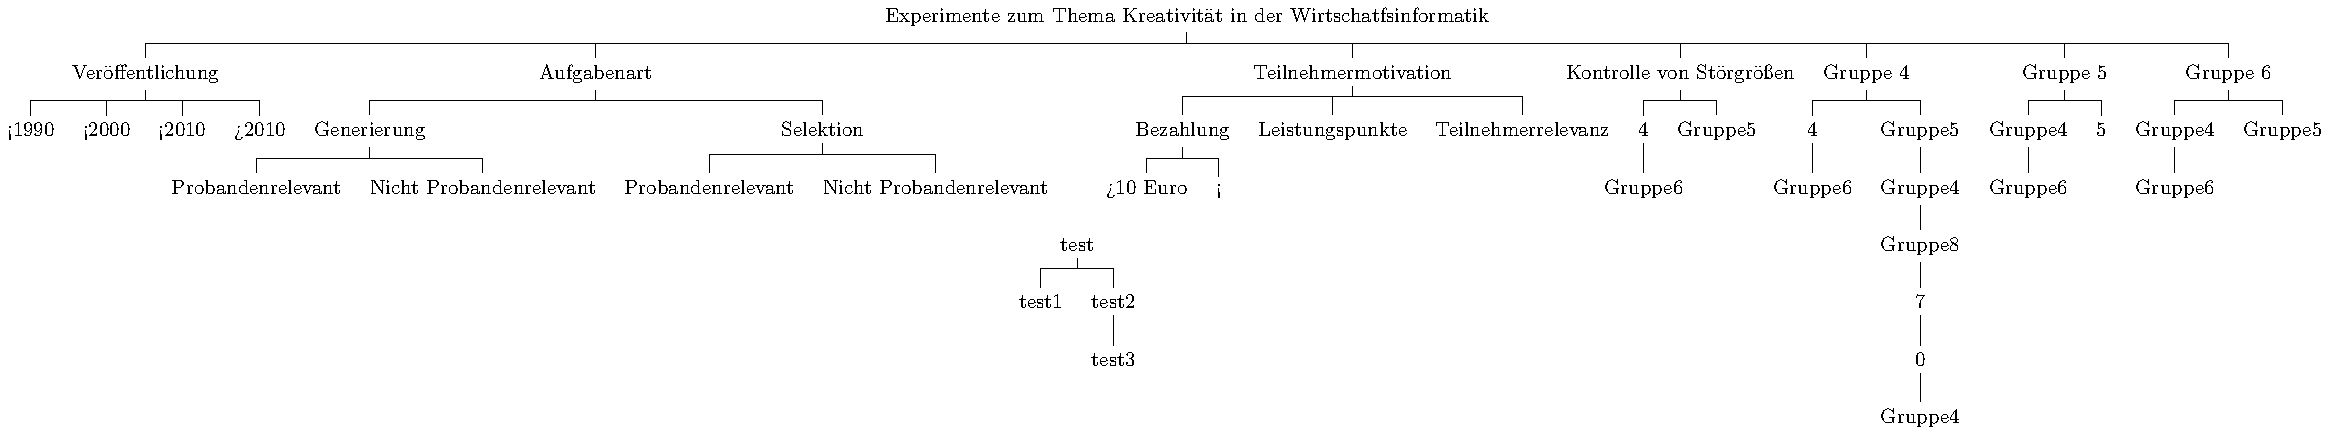
\includegraphics[width=\textheight]{_img/_forest/block_experiment.pdf}%
  \end{adjustbox}
\end{figure}

\section{Geschäftsmodelle}


\begin{mydef}{Geschäftsmodell}{def_gm}
  Im Zuge dieser Arbeit impliziert der Begriff „Wirtschaftsinformatik“ die Betrachtung (konstruierter) IT-Artefakte ausschließlich in Form softwareseitiger Anwendungssysteme.
  This theorem is numbered with  \ref{test} and is given on page \pageref{test}.
\end{mydef}
\section{Kreativität}
Es gibt in der Literatur nicht DIE Definition von Kreativität. Neben vielen Versuchen von aufstellen allgemeingültiger Definitionen (vgl. Überblcik Krea dfis) und dem forumluieren einer „standard definition of creativity) scheitern viele…

Kreativität soziale Aktivität nach Csik, daher sind Messungen nach dem Grad der kreativität oft abhängig vom jeweiligen Kontext einer jeweiligen Community und schwer zu pauschalisieren.

Die meisten Autoren sind sich jedoch darüber einig, dass kreatitivtät bedeut etwas „neus und innovatives zu schaffen“.
Innerhalb dieser Arbeit fokussieren wir uns auf 3 oft verwendete Frameworks um Kreativität zu beschreiben. Einmal Rhodes 4P. Dieses eigent sich besodners zur strukturellen und vergleichabren Darstellung von Kreativitätsmerkameln.

Guilford 4 phasen kreativer prozess: (a) preparation, (b) incubation, (c) illumination, and (d) verification
Guilford merkamel:
a)	Fluency (many ideas)
b)	Flexibilität (anders denken)
c)	Problemsensitivität (problem erkennen)
d)	Originality
e)	Elaboration
f)	Sensitivity to topic

Torrance macht daraus creativity scored on 4 scales:
Fluency. The total number of interpretable, meaningful, and relevant ideas generated in response to the stimulus.
Flexibility. The number of different categories of relevant responses.
Originality. The statistical rarity of the responses.
Elaboration. The amount of detail in the responses.

Consesnsual assement technicu

Der body of litertur innerhalb der Kreativitä ist enorm. Zudem sind Veröffentlichungen von Diskussionen vom zusammenhang IS/IT und Kreativität in den letzten Jahren stark gesteigen (CSS Shneidernmann). Bei der Vergleichdneden Betrachtung von Kreativitätsexperimenten wird diese vor diesem Hintergrund allerdings aus 3 Blickwinkeln betrachtet, welche hauptsächlich kennzeichnetnd sind: Die Eben der Kreativität, jeweilige Betrachtung welcher 4P und die Operationalisierung bzw. Messung der Kreativität. Veranschaulicht wird dieses im Würfel Abbildung 3. Betrachtet man ein kreatives Produkt kann dieses zb. aus einer Einzelleistung entstehen (Ebene Indivudal), das  Ergbnis 

\begin{mydef}{Kreativität}{def_krea}
  Im Zuge dieser Arbeit impliziert der Begriff „Wirtschaftsinformatik“ die Betrachtung (konstruierter) IT-Artefakte ausschließlich in Form softwareseitiger Anwendungssysteme.
  This theorem is numbered with  \ref{def:def_krea} and is given on page \pageref{def:def_krea}.
\end{mydef}

In der Literatur existeiert trotz vieler Versuche keine einheitliche Definition, wie sich Kreativität definieren lässt. Rhode identifizierte 1961 in diesem Zusammenhang vier Cluster, welche interaktiv auftreten können und aus denen sich das Gesamtkonstrukt der Kreativität bildet. Kreativität kann mdemanch gesehen werden als das Ergebnis kreativer Arbeit und kann selbst kreativ sein. Ein weiterer Forshungsaspket bezieht die kreative Person in den Mittelpunkt, wogegen anderen arbeiten Kreativität als einen Prozess, eine Abfolger kreativer Tätigkeiten sehen,
Diese sogenannten 4P bilden das Grundfundament und diesnen als Basis der Literaturrecherche, indem jedem Paper eine oder mehrer Dimensionen der 4Ps nach Rhode zugeweisenw erden. Alos: Liegt im Fokus des Paper die Person (inwieweit steigert die SW-Lösung die Kreativität einer Person) oder aber das Endresultat (Wie kreativ ist das Endprodukt?). Der kreative Prozess manifestiert sich dabei in erster Linie durch die Wahl der unabhänigen Variablen zb. durch den Einsatz bestimmter Kreativitätstechniken oder Prozessabfolgen.

Kreatives Produkt: Useful, Originality: Entschiedne wird das durch das Fielkd: System Model der Kreativität

Über usefullnes, Effektivität entscheiden die gatekeeper

Die Grundidee des Systemmodells nach Cisk ist jedens, dass neue Ideen um kreativ su sein nicht nu neu sein müssen, sondern auf angebracht und nützlich. Die Effektivität ist demnach durch das soziale Umfeld zu bestimmen, in dem diese neue Ideen ablehnen oder annehmen. Bein Annahme können neue Ideen dann zur bestehenden Wissensbasis (Domäne) hibnzugefügt werden.

\section{Literaturreview}

\begin{mydef}{Literaturreview}{def_lr}
  Im Zuge dieser Arbeit impliziert der Begriff „Wirtschaftsinformatik“ die Betrachtung (konstruierter) IT-Artefakte ausschließlich in Form softwareseitiger Anwendungssysteme.
  This theorem is numbered with  \ref{def:def_lr} and is given on page \pageref{def:def_lr}.
\end{mydef}

\section{Wirtschaftsinformatik}

Der Forschungsbereich der Wirtschaftsinfomratik ist stark durch die beiden paradigmischen Anstäze der Gestaltungs- sowie Verhaltenorientierung geprägt. 
Die Wirtschaftsinformatik sieht sich selbst als interdisziplinare Realwissenschaft, welche Bereiche aus der technischen Perspektive als auch aus der betriebwissenschaftlichen Sichtweise betrachtet und beide verbindet.
Streng genommen weisen die Forschungskulturen der deutschen Wirtschaftsinformatik einerseits und der angloamerikanischen Schwesterdiszplin der Information Systems andererseits große Unterschiede hinsichtlich postulierter Methoden sowie Zielpräferenzen auf. Vor dem Hintergrund der in dieser Arbeit vorrangigen Untersuchung empirischer Evaluationsmethoden ist eine strikte Trennung beider Gebiete in dieser Hinsicht allerdings nicht zwingend notwendig.  Beide Disziplinen unterscheiden zwischen den sich gegenüberstehenden Forschungsparadigmen der Gestaltungsorientierung („Design Science“ im internationalen Raum) und der Erklärungsorientierung („Behaviroul Science“). Die deutsche WI sieht sich dabei stärker auf den praxisorientierteren Gestaltungsansatz fokussiert (Relevanz), wogegen ihr internationale Vertretung den theoretisch geprägten erklärungsorientierten Ansatz in den Vordergrund stellt (Rigor).  Die Ziele der Verhaltensorientierung sind vor allem die des Erklärens und Beschreibens von Zusammenhängen und Theorien (Wahrheitsfindung). Die Hauptfelder gestaltungsorientierter Wirtschaftsinformatik liegen hingegen in der Schaffung und Evaluierung zweckmäßiger Artefakte. Ziel von Design Science ist die Schaffung und Evaluierung zweckbezogener Artefakte zur Lösung von Organisationsproblemen (Simon?) {Frank 1999 69} Ziel dieser Artefakte ist es, bereits vorhandene Anwendungssysteme zu erweitern oder Probleme zu lösen, die entweder durch informationstechnische Anwendungen zuvor nicht zufriedenstellend gelöst wurden oder konnten. Die Gestaltungsorienteirete Forschung liefert dazu neue Lösungen als IT Artefakt, etwa in Form von Softwareprotytypen, deren Nutzen es im Prozess durch Anwendung geeigneter Forschungsmethoden zu evaluieren gilt. Dabei treten beide Forschungsparadigmen nicht streng dichotom auf, sondern können und müssen sich synergetisch ergänzen. Gerade im Zusammenhang mit dem langen geführten Diskurs zwischen Rigor und Relevanz zeigte sich, dass sich die deutsche Wirtschatfsinformatik zu stark auf den  \label{test}praxisnahen gestaltungsorientioerten Ansatz besinnte. Einerseits wird dieses Vorgehen von vielen Autoren gelobt (Momerndum für die gestatungsorientioere WInfo), andereseits wird auch oft das fehlende theoretische Fundament bemängelt. Gerade im Vergleich zur internationaen Wirtschaftsinformatik, welche sich stärker auf die theorethscihe fundierung bedacht ist, herrsche in der deutschen WI nachholbedarf. Auch die internationale Wi rief mit ihrer klaren Positionierung zur theoretischen Empirie zum Diskurs auf, sprach ihrerseits sogar von einer Identitäskrise (Benbasat und Zmud). Benbast und Zmud kritisierten diesen Fokus und verlangte danach, dass IT-Artefakt in den Mittelpunkt zu stellen und sich auf die Konstruktion nützlicher zu besinnen: Focus should be on how to best design IT artifacts and IS systems to increase their compatibility, usefulness, and ease of use or on how to best manage and support IT or IT-enabled business initiatives.
Das gemeinschaftliche Ziel der deutschen sowie internationalen Wirtschaftsinformatik besteht daher in der Sicherstellung und Steigerung der „Relevanz und Rigor“ Prämisse, also der praxisorientierten gestalterischen Artefaktentwicklung (Gestaltungsorientiert) sowie gleichzeitiger Korrektheit durch Prüfung mittles angemessener theoretischer Fundierung (Erklärungsorientiert). {Alturki 2012 32: 313} In Anbetracht dieses Ziels gilt es als Aufgabe der Wirtschaftsinfomratik das  richtige Verhältniss im Nutzen beider Forschungsansätze zu finden und implementieren. {Becker 2008 239: 5}

Der erforderliche Evaluationsschritt innerhalb der DesignScience versucht die Nützlichkeit eines Artefaktes zu „erklären“. Dieser Vorgang ist definitionsgemäß der Behavirolistischen Orientierung zuzuschreiben. Dadurch finden dessen verfügbaren Methoden implizit auch im Gestaltungsprozess Anwendung.  


In der Vergangenheit wurden eine Vielzahl möglicher Klassifikation von IT-Artefakten vorgenommen (Alter?) Die in diesem Zusammenhang jedoch meist genutze war die von HamrchSmith und Hevner dargestellte Unterschidung der Artefakte in: Konstrukte, Modelle, Methode, Instantiierung.
Bei der Definition eines IT-Artefaktes herrscht nach Alter kein kohärentes Verständnis über die genaue Definition eines IT-Atefaktes entwickelt hat, so sprechen sich viele für die von Simon postulierten Definition nach den Arten von Artefakte aus. Diese stellen sich demnachin Form von Konstrukten, Modellen, Methoden oder instatiierungen dar.
Nach Wotawa u. Thierau 1990 kennzeichnet sich die Evaluirung dieser Artefakte durch eine systematische Tätigkeit, welche eine Bewertung einer Sache (Artefakt) nach zweckgerichteter Form vornimmt. Somit dient die Artefaktevaluaiton vornehmlich der Feststellung jender „Nützlichkeit“.

Hess stellte diesen Vorgang schematisch wie in Fig 3 dargestellt auf:




\vspace{1cm}


\begin{mydef}{Wirtschaftsinformatik}{def_wi}
  Im Zuge dieser Arbeit impliziert der Begriff „Wirtschaftsinformatik“ die Betrachtung (konstruierter) IT-Artefakte ausschließlich in Form softwareseitiger Anwendungssysteme.
  This theorem is numbered with  \ref{def:def_wi} and is given on page \pageref{def:def_wi}.
\end{mydef}


\begin{tikzpicture}
\begin{axis} [axis x line=bottom, axis y line = left, grid, width=\textwidth,
]
\addplot coordinates {(0,4) (3,7)};
\fill[blue, opacity=.1] (0,5) rectangle (3,5.5);
\end{axis}
\end{tikzpicture}

\begin{tikzpicture}
\begin{axis}
\addplot coordinates {(0,4) (3,7)};
\end{axis}
\end{tikzpicture}

 
\begin{figure}[h]
 \centering
 %\resizebox{\textwidth}{!}{%
 \IfFileExists{../../_preamble/check_file.tex}% prüfen aus welcher datei der aufruf stattfindet
{%
\providecommand{\myPath}{../../}% file exists=true: befinde mich im unterverzeichnis
}%
{%
\providecommand{\myPath}{}% file exists=false: befinde mich im root_verzeichnis
}%
\documentclass[tikz]{standalone}
%% läd standalone-klasse mit tikz-argument
%//Tikzbibliotheken\\%
\usetikzlibrary{						% Bibliotheken zur direkten Einbindung in TIKZEdt
arrows, 
fit,
shapes.geometric, 
matrix,
calc,
decorations.markings,
decorations.pathreplacing,
decorations.pathmorphing,
backgrounds,
shadings, 
shadows,
positioning,
mindmap,
trees,
datavisualization
}%% diverse tikz-bibliotheken
%%Font etc.%%
\usepackage{lmodern}					% OK, Latin Modern font,											check: 25.08.18
\usepackage{xcolor} 					% OK, Definieren und Nutzen von versch. Farben						check: 25.08.18
\usepackage{graphicx}					% OK, Bereitstellen von \includegraphics							check: 25.08.18

%%Forest%%
\usepackage{forest}						% OK, Baumdarstellung aus dem linguistischen Bereich				check: 25.08.18
\useforestlibrary{edges}

%%Venndiagramm%%
\usepackage{venndiagram}				% OK, Definieren und Darstellen von Venndiagrammen					check: 25.08.18

%%Tabellen%%
\usepackage{booktabs}					% OK, Schönere Tabellen ohne vertikale Linien \toprule etc.			check: 25.08.18
\usepackage{tabularx}					% OK, Weiterer Spaltentyp passt Tabellenbreite  automatisch an		check: 25.08.18
\usepackage{multirow}					% OK, Zellenspannung über mehrere Zeilen							check: 25.08.18
%\usepackage{makecell}					% OK, Tabellenlayout (Tabaellenheader) ähnlich \multirow			check: 25.08.18
\usepackage{tablefootnote}				% OK, Fußnoten in Tabellen (\footnote funktioniert nicht)			check: 25.08.18
\usepackage{array} 						% OK, Erstellen eigener Columntypen in Tabellenumgebungen			check: 25.08.18

%%Grafiken und Plots%%
\usepackage{tikz} 						% OK, Natives zeichnen in Latex ,									check: 25.08.18
\usepackage{tikz-cd} 					% OK, Erstellen von kommutativen Diagrammen in Tikz,				check: 25.08.18
\usepackage{pgfplots}					% OK, Plotten von Daten,											check: 25.08.18
\pgfplotsset{compat=newest}				% OK, Einstellen der Kompatibilitätsversion,						check: 25.08.18
\usepackage{pgfplotstable}				% OK, Plotten und schreiben von Daten in Tabellen,					check: 25.08.18
\usepackage{pgfcalendar} 				% OK, Umrechnen von Datumskoordinaten,								check: 25.08.18
\usepgfplotslibrary{dateplot}			% OK, Plotten von Datumskoordinaten,								check: 25.08.18
\usepgfplotslibrary{units}				% OK, Darstellen von Einheiten als Achsenlabel,						check: 25.08.18%% nur laden wenn weitere graphic pakete benötigt werden (tabellen, pgfplot,...)
%%define tikz-stlyes here, colours etc.
\tikzset{
block_phantom/.style={block_normal, draw=red, fill=none},
block_phantom/.style={block_normal, draw=blue, fill=none}
}
%\tikzstyle{block_phantom}=[block_normal, draw=red, fill=none]%% tikz-styles, farben etc.
\usepackage{pgfplots}
\usepackage{pgfplotstable}
\usepgfplotslibrary{dateplot}
\usepgfplotslibrary{units}
\usepackage{pgfcalendar} 
%%Kompatibilitäts-Version%%
\pgfplotsset{compat=newest}%% tikz-styles, farben etc.
\pgfplotsset{
  global_appearance/.style={
  grid_appearance,
  scale only axis,
  width= .75\textwidth,
  %width=12.5cm, % 13,5
  height=.4\textwidth
  }
}

\pgfplotsset{
  grid_appearance/.style={
   grid,
   grid style = {loosely dotted , thin},
  }
}

\pgfplotsset{
 %every axis plot/.append style={no markers},
  every pin/.append style={font=\footnotesize },
  every mark/.append style={scale=3},
  legend style=
  {
  font=\tiny, 
  %draw=none, 
  cells={align=left}, 
  at={(0.5,1.00)},
  anchor=north,
 % legend pos= north west
  },
  legend columns = 2,
  label style={font=\scriptsize},
  tick label style={font=\tiny},
}

\pgfplotsset{
  tuftle_like_axes/.style={
  thin,  %vorher semithick
  tick style={major tick length=4pt,thin,black}, %vorher semithick
  separate axis lines,
  axis x line*=bottom,
  axis x line shift=10pt,
  xlabel shift=5pt,
  axis y line*=left,
  axis y line shift=10pt,
  tick align = outside,
  ylabel shift=2pt,
  enlarge y limits=false,
  enlarge x limits=false,
  }
}

%%Tufte-Design%%
% \makeatletter
% \pgfplotsset{
  % tufte axes/.style =
    % {
      % after end axis/.code =
        % {
          % \draw ({rel axis cs:0,0} -| {axis cs:\pgfplots@data@xmin,0}) -- ({rel axis cs:0,0}  -| {axis cs:\pgfplots@data@xmax,0});
          % \draw ({rel axis cs:0,0} |- {axis cs:0,\pgfplots@data@ymin}) -- ({rel axis cs:0,0}  |-{axis cs:0,\pgfplots@data@ymax});
        % },
      % axis line style = {draw = none},
      % tick align      = outside,
      % tick pos        = left
    % }
% }
% \makeatother%% tikz-styles, farben etc.
\begin{document}%
\IfFileExists{../../_preamble/check_file.tex}% prüfen aus welcher datei der aufruf stattfindet
{%file exists=true: befinde mich im unterverzeichnis
\IfFileExists{data/check_file.tex}% aus welcher datei der aufruf stattfindet
 	{\pgfplotstableread[]{data/plot_gm_gmi.dat}\data}
 	{\pgfplotstableread[]{_img/_pgfplot/data/plot_gm_gmi.dat}\data}
% add new column with Julian integer numbers
% therefore a counter is needed
    \newcount\julianday
    \pgfplotstablecreatecol[
        create col/assign/.code={
            % convert the number of the current row and save it to `\julianday'
            \pgfcalendardatetojulian{\thisrow{year}}{\julianday}
            % then give the entry of `\julianday' to `\entry' which is then
            % given to the current cell
            \edef\entry{\the\julianday}
            \pgfkeyslet{/pgfplots/table/create col/next content}\entry
        },
    ]{JulianDay}{\data}
    % because the `dateplot' library shifts automatically all dates to 0 using
    % the first found coordinate we can't use the created `JulianDay' data
    % directly for `linear regression', but have to do the same first with
    % the data
        % get the first coordinate of the column ...
        \pgfplotstablegetelem{0}{JulianDay}\of{\data}
        % ... and store it in `\xmin'
        \pgfmathtruncatemacro{\xmin}{\pgfplotsretval}
    % now create another column with the shifted values
    \pgfplotstablecreatecol[
        expr={\thisrow{JulianDay}-\xmin},
    ]{JulianDayMod}{\data}

\begin{tikzpicture}
\begin{axis} [ 
width=\textwidth,
date coordinates in = x,
date ZERO = 1972-01-01,
xmin = 1980-01-01,
xmax = 2015-01-01,
%xtick distance=10,
%try min ticks = 5,
xticklabel=\year,
global_appearance,
tuftle_like_axes,
xlabel={},
ylabel={Anzahl Ver\"offentlichungen [St\"uck]},
%xtick={data},
 xtick={
%1972-01-01, 
%1974-01-01, 
1976-01-01, 
%1978-01-01, 
1980-01-01, 
%1982-01-01,
1984-01-01,
%1986-01-01,
1988-01-01,
%1990-01-01,
1992-01-01,
%1994-01-01,
1996-01-01,
%1998-01-01,
2000-01-01,
2001-01-01,
2002-01-01,
2003-01-01,
2004-01-01,
2005-01-01,
2006-01-01,
2007-01-01,
2008-01-01,
2009-01-01,
2010-01-01,
2011-01-01,
2012-01-01,
2013-01-01,
2014-01-01,
2015-01-01},
%ytick={-50, 0, 200, 400, 600, 800},
ymin=0,
ymax=830,
x tick label style={rotate=45,anchor=north east}
% x unit=\si{},
 %y unit=\si{},
]
\IfFileExists{data/check_file.tex}% aus welcher datei der aufruf stattfindet
{%
\addplot [thin]table [x=year, y=gm]{data/plot_gm_gmi.dat};%
\addplot [densely dashed,  thin ]table [x=year, y=gmi]{data/plot_gm_gmi.dat};%
}%
{%
\addplot [thin]table [x=year, y=gm]{_img/_pgfplot/data/plot_gm_gmi.dat};%
\addplot [densely dashed, thin ]table [x=year, y=gmi]{_img/_pgfplot/data/plot_gm_gmi.dat};%
}%

\addplot[black, opacity=1, very thin,mark=halfsquare right*, mark options={color=black, scale=1}] table [x=year,y={create col/linear regression={x=JulianDayMod,y=gm}}]{\data};%%Regressionslinie
\addplot[black, opacity=1, very thin, mark=halfsquare left*,mark options={color=black, scale=1}] table [x=year,y={create col/linear regression={x=JulianDayMod,y=gmi}}]{\data};%%Regressionslinie

\addlegendentry{Gesch\"aftsmodell};
\addlegendentry{Gesch\"aftsmodell-\\innovation};
\addlegendentry{Regression GM};
\addlegendentry{Regression GMI};
%\node [pin=90: \footnotesize Regression Gesch\"aftsmodell] at (2000-01-01,255) {};
%\node [pin=-90: \footnotesize Regression Gesch\"aftsmodellinnovation] at (2011-01-01,105) {};
%\fill[blue, opacity=.1] (1984-01-01,6) rectangle (2015-01-01,800);
%\fill[blue, opacity=.1] (1984-01-01,0) rectangle (2015-01-01,200);
%\draw[black, opacity=1] (1984-01-01,0) to (2015-01-01,200);
%\draw[black, opacity=1, densely dashdotted] (1984-01-01,6) to (2015-01-01,800);
\end{axis}%
\end{tikzpicture}%
%
}%
{%file exists=false: befinde mich im root_verzeichnis
\IfFileExists{data/check_file.tex}% aus welcher datei der aufruf stattfindet
 	{\pgfplotstableread[]{data/plot_gm_gmi.dat}\data}
 	{\pgfplotstableread[]{_img/_pgfplot/data/plot_gm_gmi.dat}\data}
% add new column with Julian integer numbers
% therefore a counter is needed
    \newcount\julianday
    \pgfplotstablecreatecol[
        create col/assign/.code={
            % convert the number of the current row and save it to `\julianday'
            \pgfcalendardatetojulian{\thisrow{year}}{\julianday}
            % then give the entry of `\julianday' to `\entry' which is then
            % given to the current cell
            \edef\entry{\the\julianday}
            \pgfkeyslet{/pgfplots/table/create col/next content}\entry
        },
    ]{JulianDay}{\data}
    % because the `dateplot' library shifts automatically all dates to 0 using
    % the first found coordinate we can't use the created `JulianDay' data
    % directly for `linear regression', but have to do the same first with
    % the data
        % get the first coordinate of the column ...
        \pgfplotstablegetelem{0}{JulianDay}\of{\data}
        % ... and store it in `\xmin'
        \pgfmathtruncatemacro{\xmin}{\pgfplotsretval}
    % now create another column with the shifted values
    \pgfplotstablecreatecol[
        expr={\thisrow{JulianDay}-\xmin},
    ]{JulianDayMod}{\data}

\begin{tikzpicture}
\begin{axis} [ 
width=\textwidth,
date coordinates in = x,
date ZERO = 1972-01-01,
xmin = 1980-01-01,
xmax = 2015-01-01,
%xtick distance=10,
%try min ticks = 5,
xticklabel=\year,
global_appearance,
tuftle_like_axes,
xlabel={},
ylabel={Anzahl Ver\"offentlichungen [St\"uck]},
%xtick={data},
 xtick={
%1972-01-01, 
%1974-01-01, 
1976-01-01, 
%1978-01-01, 
1980-01-01, 
%1982-01-01,
1984-01-01,
%1986-01-01,
1988-01-01,
%1990-01-01,
1992-01-01,
%1994-01-01,
1996-01-01,
%1998-01-01,
2000-01-01,
2001-01-01,
2002-01-01,
2003-01-01,
2004-01-01,
2005-01-01,
2006-01-01,
2007-01-01,
2008-01-01,
2009-01-01,
2010-01-01,
2011-01-01,
2012-01-01,
2013-01-01,
2014-01-01,
2015-01-01},
%ytick={-50, 0, 200, 400, 600, 800},
ymin=0,
ymax=830,
x tick label style={rotate=45,anchor=north east}
% x unit=\si{},
 %y unit=\si{},
]
\IfFileExists{data/check_file.tex}% aus welcher datei der aufruf stattfindet
{%
\addplot [thin]table [x=year, y=gm]{data/plot_gm_gmi.dat};%
\addplot [densely dashed,  thin ]table [x=year, y=gmi]{data/plot_gm_gmi.dat};%
}%
{%
\addplot [thin]table [x=year, y=gm]{_img/_pgfplot/data/plot_gm_gmi.dat};%
\addplot [densely dashed, thin ]table [x=year, y=gmi]{_img/_pgfplot/data/plot_gm_gmi.dat};%
}%

\addplot[black, opacity=1, very thin,mark=halfsquare right*, mark options={color=black, scale=1}] table [x=year,y={create col/linear regression={x=JulianDayMod,y=gm}}]{\data};%%Regressionslinie
\addplot[black, opacity=1, very thin, mark=halfsquare left*,mark options={color=black, scale=1}] table [x=year,y={create col/linear regression={x=JulianDayMod,y=gmi}}]{\data};%%Regressionslinie

\addlegendentry{Gesch\"aftsmodell};
\addlegendentry{Gesch\"aftsmodell-\\innovation};
\addlegendentry{Regression GM};
\addlegendentry{Regression GMI};
%\node [pin=90: \footnotesize Regression Gesch\"aftsmodell] at (2000-01-01,255) {};
%\node [pin=-90: \footnotesize Regression Gesch\"aftsmodellinnovation] at (2011-01-01,105) {};
%\fill[blue, opacity=.1] (1984-01-01,6) rectangle (2015-01-01,800);
%\fill[blue, opacity=.1] (1984-01-01,0) rectangle (2015-01-01,200);
%\draw[black, opacity=1] (1984-01-01,0) to (2015-01-01,200);
%\draw[black, opacity=1, densely dashdotted] (1984-01-01,6) to (2015-01-01,800);
\end{axis}%
\end{tikzpicture}%
\\%\\
%\begin{tikzpicture}
\begin{axis}[
ybar interval,
global_appearance,
tuftle_like_axes,
ymax=800,
ymin=0, 
ybar interval=1, 
date coordinates in = x,  
date ZERO = 1988-01-01, 
xmax = 2014-12-31, 
x tick label style={rotate=90,anchor=east},
%minor y tick num = 5,
ylabel = Anzahl Veröffentlichungen,
xticklabel=\year,
height=\axisdefaultheight,
]

\IfFileExists{data/check_file.tex}% aus welcher datei der aufruf stattfindet
{%
\addplot [thin]table [x=year, y=gm]{data/plot_gm_gmi.dat};%
\addplot [densely dashed,  thin ]table [x=year, y=gmi]{data/plot_gm_gmi.dat};%
}%
{%
\addplot [thin]table [x=year, y=gm]{_img/_pgfplot/data/plot_gm_gmi.dat};%
\addplot [densely dashed, thin ]table [x=year, y=gmi]{_img/_pgfplot/data/plot_gm_gmi.dat};%
}%
\end{axis}
\end{tikzpicture}%\\
}%
\end{document}%
%
 %}
 \caption{}
 \end{figure}
 
 

\input{\myPath_text/1_mainmatter/030_meta_rq1.tex}
\input{\myPath_text/1_mainmatter/031_literaturreview_identifikation.tex}
\input{\myPath_text/1_mainmatter/032_literaturreview_analyse.tex}
\input{\myPath_text/1_mainmatter/040_meta_rq2.tex}
\input{\myPath_text/1_mainmatter/041_ergebnisse_implikationen.tex}

% \printbibliography
%\input{text/anhang} % Anhänge
\end{onehalfspace} %Ende 1,5-facher Zeilenabstand


\end{document}
